\documentclass[11pt]{article}
\usepackage[margin=1in]{geometry}
\usepackage[T1]{fontenc}
\usepackage[utf8]{inputenc}
\usepackage{lmodern}
\usepackage{microtype}
\usepackage{graphicx}
\usepackage{booktabs}
\usepackage{tabularx}
\usepackage{array}
\usepackage{longtable}
\usepackage{xcolor}
\usepackage{amsmath}
\usepackage{caption}
\usepackage{enumitem}
\usepackage{url}
\usepackage[hidelinks]{hyperref}
\usepackage[numbers,sort&compress]{natbib}
\usepackage{authblk}
\usepackage{titlesec}
\usepackage{ragged2e}
\usepackage{setspace}
\usepackage{fancyhdr}
\usepackage{placeins}

\definecolor{accent}{RGB}{35,75,120}
\titleformat{\section}{\large\bfseries\color{accent}}{\thesection.}{0.5em}{}
\titleformat{\subsection}{\normalsize\bfseries}{\thesubsection}{0.5em}{}
\setlength{\parindent}{0.45cm}
\setlength{\parskip}{0.15em}
\setlength{\headheight}{14pt}
\setlength{\emergencystretch}{2em}
\renewcommand{\arraystretch}{1.15}
\newcolumntype{Y}{>{\RaggedRight\arraybackslash}X}
\captionsetup{font=small,labelfont=bf}
\pagestyle{fancy}
\fancyhf{}
\fancyhead[L]{Structural templates, protein stability and tetrapod longevity}
\fancyfoot[C]{\thepage}
\hypersetup{pdftitle={The choice of structural template can create apparent links between predicted protein stability and longevity in tetrapods}}

% Numbers and table bodies generated from the result files of each study (M = mammals, R = reptiles and amphibians)
% from PROTEINAS_LONGEVIDAD\paper\generated\numbers.tex
% Generated by src/11_paper_tables.py from results/*.json. Do not edit by hand.
\newcommand{\MNSpecies}{57}
\newcommand{\MNGenes}{1,755}
\newcommand{\MNGenAge}{204}
\newcommand{\MNBackground}{1,547}
\newcommand{\MNGenesOpossum}{1,503}
\newcommand{\MPOneBeta}{$-$0.075}
\newcommand{\MPOneLo}{$-$0.183}
\newcommand{\MPOneHi}{0.033}
\newcommand{\MPOneP}{0.178}
\newcommand{\MPOneLambda}{0.97}
\newcommand{\MPTwoBeta}{$-$0.047}
\newcommand{\MPTwoLo}{$-$0.126}
\newcommand{\MPTwoHi}{0.032}
\newcommand{\MPTwoP}{0.264}
\newcommand{\MPTwoCompP}{0.774}
\newcommand{\MPTwoNullMean}{$-$0.064}
\newcommand{\MPTwoNullSD}{0.022}
\newcommand{\MOpBeta}{0.014}
\newcommand{\MOpLo}{$-$0.038}
\newcommand{\MOpHi}{0.067}
\newcommand{\MOpP}{0.595}
\newcommand{\MOpCompP}{0.750}
\newcommand{\MOpDetect}{18}
\newcommand{\MMainDetect}{42}
\newcommand{\MRBeta}{$-$0.137}
\newcommand{\MRLo}{$-$0.252}
\newcommand{\MRHi}{$-$0.021}
\newcommand{\MRP}{0.026}
\newcommand{\MNP}{0.06}
\newcommand{\MNNBeta}{$-$0.028}
\newcommand{\MNNP}{0.63}
\newcommand{\MNNOpBeta}{0.126}
\newcommand{\MNNOpP}{0.23}
\newcommand{\MExPrimBeta}{0.036}
\newcommand{\MExPrimLo}{$-$0.020}
\newcommand{\MExPrimHi}{0.091}
\newcommand{\MExHumBeta}{$-$0.011}
\newcommand{\MExHumP}{0.82}
\newcommand{\MAdjRBeta}{$-$0.032}
\newcommand{\MAdjRP}{0.58}
\newcommand{\MOLSP}{$<$0.001}
\newcommand{\MPostBetaMin}{$-$0.090}
\newcommand{\MPostBetaMax}{$-$0.065}
\newcommand{\MPostPMin}{0.12}
\newcommand{\MPostPMax}{0.25}
\newcommand{\MMouseSiteR}{0.91}
\newcommand{\MMouseSpeciesR}{0.74}
\newcommand{\MMouseBetaHuman}{$-$0.024}
\newcommand{\MMouseBetaMouse}{$-$0.004}
\newcommand{\MCOneObs}{0.29}
\newcommand{\MCOneAlt}{0.64}
\newcommand{\MCOneFrac}{97.3}
\newcommand{\MCTwoBur}{1.36}
\newcommand{\MCTwoExp}{0.60}
\newcommand{\MCTwoFrac}{96.3}
\newcommand{\MGenesTested}{1,478}
\newcommand{\MGenesPos}{41.7}
\newcommand{\MEGenes}{1,341}
\newcommand{\MEOffHum}{$-$1.96}
\newcommand{\MEOffOpo}{$-$0.73}
\newcommand{\MEOffPla}{$-$0.62}
\newcommand{\MEaEst}{$-$1.34}
\newcommand{\MEaLo}{$-$1.80}
\newcommand{\MEaHi}{$-$1.04}
\newcommand{\MEaVerdict}{confirmed}
\newcommand{\MEbEst}{0.42}
\newcommand{\MEbLo}{0.30}
\newcommand{\MEbHi}{0.59}
\newcommand{\MErOpPl}{0.99}
\newcommand{\MErHuPl}{0.56}
\newcommand{\MErHuOp}{0.62}
\newcommand{\MEbVerdict}{confirmed}
\newcommand{\MEcBeta}{0.010}
\newcommand{\MEcLo}{$-$0.039}
\newcommand{\MEcHi}{0.060}
\newcommand{\MEcP}{0.701}
\newcommand{\MEcVerdict}{replicated}
\newcommand{\MEBetaHum}{$-$0.081}
\newcommand{\MEBetaOpo}{0.010}
\newcommand{\MERankHum}{1}
\newcommand{\MERankOpo}{2}
\newcommand{\MERankPla}{1}
\newcommand{\MECompP}{0.906}

% from PROTEINAS_LONGEVIDAD\paper\generated\posthoc.tex
% Generated by src/14_posthoc_tables.py (amendment E6, post hoc). Do not edit by hand.
\newcommand{\MSixGenesIn}{1,341}
\newcommand{\MSixGenes}{1,321}
\newcommand{\MSixPost}{0.974}
\newcommand{\MSixOffMsa}{$-$0.52}
\newcommand{\MSixOffMsaLo}{$-$0.87}
\newcommand{\MSixOffMsaHi}{$-$0.09}
\newcommand{\MSixRankMsa}{4}
\newcommand{\MSixOffMsaHs}{$-$0.61}
\newcommand{\MSixOffMsaHsLo}{$-$0.94}
\newcommand{\MSixOffMsaHsHi}{$-$0.20}
\newcommand{\MSixRankMsaHs}{3}
\newcommand{\MSixOffHum}{$-$1.96}
\newcommand{\MSixOffHumLo}{$-$1.99}
\newcommand{\MSixOffHumHi}{$-$1.92}
\newcommand{\MSixRankHum}{1}
\newcommand{\MSixOffPla}{$-$0.60}
\newcommand{\MSixOffPlaLo}{$-$0.91}
\newcommand{\MSixOffPlaHi}{$-$0.19}
\newcommand{\MSixRankPla}{2}
\newcommand{\MSixDiffMsaPla}{0.07}
\newcommand{\MSixDiffMsaPlaLo}{$-$0.08}
\newcommand{\MSixDiffMsaPlaHi}{0.22}
\newcommand{\MSixDiffMsaHum}{1.44}
\newcommand{\MSixDiffMsaHumLo}{1.10}
\newcommand{\MSixDiffMsaHumHi}{1.87}
\newcommand{\MSixDiffHsMsa}{$-$0.09}
\newcommand{\MSixDiffHsMsaLo}{$-$0.15}
\newcommand{\MSixDiffHsMsaHi}{$-$0.03}
\newcommand{\MSixRPla}{0.993}
\newcommand{\MSixRHum}{0.52}
\newcommand{\MSixBeta}{0.013}
\newcommand{\MSixLo}{$-$0.035}
\newcommand{\MSixHi}{0.062}
\newcommand{\MSixP}{0.56}

% from PROTEINAS_LONGEVIDAD\paper\generated\PrimaryRows.tex
\newcommand{\MPrimaryRows}{%
P1: all genes, human template & $-$0.075 & [$-$0.183, 0.033] & 0.97 & 0.178 \\
P2: GenAge genes, human template & $-$0.047 & [$-$0.126, 0.032] & 0.98 & 0.264 \\
P2 competitive: GenAge vs 1,000 background sets & -- & -- & -- & 0.774$^{a}$ \\
\midrule
Divergence from ancestor per site (secondary) & $-$0.137 & [$-$0.252, $-$0.021] & 0.97 & 0.026 \\
Net $\Delta\Delta G$ per site (secondary) & $-$0.106 & [$-$0.216, 0.003] & 0.97 & 0.060 \\
\midrule
P1, opossum template (post hoc) & 0.014 & [$-$0.038, 0.067] & 0.97 & 0.595 \\
P2, opossum template (post hoc) & $-$0.006 & [$-$0.048, 0.036] & 0.97 & 0.780 \\
P2 competitive, opossum template (post hoc) & -- & -- & -- & 0.750$^{a}$ \\
\midrule
P1, platypus template, common sites (confirmatory, H5c) & 0.010 & [$-$0.039, 0.060] & 0.97 & 0.701 \\
P2 competitive, platypus template, common sites & -- & -- & -- & 0.906$^{a}$ \\
}

% from PROTEINAS_LONGEVIDAD\paper\generated\SensitivityRows.tex
\newcommand{\MSensitivityRows}{%
$\lambda$ fixed at 1 & 57 & $-$0.075 & [$-$0.184, 0.034] & 1.00 & 0.17 \\
No window mask & 57 & $-$0.040 & [$-$0.090, 0.009] & 0.99 & 0.11 \\
Sites with pLDDT $\geq$ 90 & 57 & $-$0.062 & [$-$0.165, 0.041] & 0.97 & 0.23 \\
Buried sites only & 57 & $-$0.060 & [$-$0.160, 0.040] & 0.97 & 0.24 \\
Exposed sites only & 57 & $-$0.116 & [$-$0.236, 0.004] & 0.98 & 0.058 \\
Primates excluded & 43 & 0.036 & [$-$0.020, 0.091] & 0.98 & 0.21 \\
\emph{Homo sapiens} excluded & 56 & $-$0.011 & [$-$0.109, 0.087] & 0.99 & 0.82 \\
Bats excluded & 54 & $-$0.071 & [$-$0.176, 0.034] & 0.94 & 0.18 \\
AnAge quality ``high'' only & 15 & $-$0.127 & [$-$0.319, 0.064] & 0.97 & 0.17 \\
Rodents excluded & 42 & $-$0.096 & [$-$0.210, 0.018] & 0.93 & 0.097 \\
Adjusted for log$_{10}$ divergence from ancestor & 57 & $-$0.032 & [$-$0.146, 0.082] & 0.97 & 0.58 \\
Background genes only & 57 & $-$0.075 & [$-$0.184, 0.034] & 0.97 & 0.17 \\
Response log$_{10}$ LQ (no mass term) & 57 & $-$0.069 & [$-$0.178, 0.041] & 0.97 & 0.21 \\
OLS with HC3 errors (no phylogeny) & 57 & $-$0.107 & [$-$0.159, $-$0.055] & -- & $<$0.001 \\
20 posterior trees (range) & 57 & $-$0.090 to $-$0.065 & -- & -- & 0.12--0.25 \\
}

% from PROTEINAS_LONGEVIDAD\paper\generated\SpeciesRows.tex
\newcommand{\MSpeciesRows}{%
\emph{Bison bison} & Artiodactyla & 33.5 & 630,000 & 0.89 & S & 0.229 & 0.223 & 0.0441 \\
\emph{Bos grunniens} & Artiodactyla & 26.3 & 667,000 & 0.69 & S & 0.224 & 0.215 & 0.0454 \\
\emph{Camelus dromedarius} & Artiodactyla & 28.4 & 434,000 & 0.80 & S & 0.235 & 0.229 & 0.0408 \\
\emph{Capra hircus} & Artiodactyla & 20.8 & 61,000 & 0.79 & S & 0.226 & 0.217 & 0.0456 \\
\emph{Ovis aries} & Artiodactyla & 22.8 & 80,000 & 0.83 & S & 0.215 & 0.210 & 0.0444 \\
\emph{Sus scrofa} & Artiodactyla & 27 & 130,000 & 0.91 & I & 0.217 & 0.214 & 0.0413 \\
\emph{Ailuropoda melanoleuca} & Carnivora & 36.8 & 117,500 & 1.26 & I & 0.229 & 0.231 & 0.0385 \\
\emph{Canis lupus} & Carnivora & 20.6 & 26,625 & 0.89 & S & 0.217 & 0.213 & 0.0377 \\
\emph{Mustela putorius} & Carnivora & 11.1 & 809 & 0.82 & S & 0.219 & 0.217 & 0.0403 \\
\emph{Neovison vison} & Carnivora & 11.4 & 925 & 0.82 & S & 0.215 & 0.213 & 0.0396 \\
\emph{Panthera leo} & Carnivora & 28 & 175,000 & 0.90 & S & 0.222 & 0.223 & 0.0368 \\
\emph{Panthera pardus} & Carnivora & 27.3 & 53,750 & 1.06 & I & 0.221 & 0.221 & 0.0368 \\
\emph{Panthera tigris} & Carnivora & 26.3 & 119,700 & 0.90 & S & 0.251 & 0.248 & 0.0379 \\
\emph{Ursus americanus} & Carnivora & 34 & 154,250 & 1.12 & I & 0.237 & 0.238 & 0.0380 \\
\emph{Ursus maritimus} & Carnivora & 43.8 & 475,000 & 1.21 & I & 0.250 & 0.247 & 0.0390 \\
\emph{Vulpes vulpes} & Carnivora & 21.3 & 4,132 & 1.22 & I & 0.222 & 0.218 & 0.0380 \\
\emph{Balaenoptera musculus} & Cetacea & 110 & 136,000,000 & 1.28 & I & 0.248 & 0.246 & 0.0410 \\
\emph{Delphinapterus leucas} & Cetacea & 40 & 1,430,000 & 0.94 & I & 0.252 & 0.247 & 0.0415 \\
\emph{Monodon monoceros} & Cetacea & 50 & 1,250,000 & 1.20 & I & 0.251 & 0.248 & 0.0414 \\
\emph{Physeter macrocephalus} & Cetacea & 77 & 28,500,000 & 1.14 & I & 0.254 & 0.255 & 0.0412 \\
\emph{Tursiops truncatus} & Cetacea & 51.6 & 200,000 & 1.63 & L & 0.269 & 0.266 & 0.0427 \\
\emph{Myotis lucifugus} & Chiroptera & 34 & 10 & 4.90 & L & 0.238 & 0.231 & 0.0473 \\
\emph{Pteropus vampyrus} & Chiroptera & 20.9 & 872 & 1.52 & L & 0.264 & 0.258 & 0.0439 \\
\emph{Rhinolophus ferrumequinum} & Chiroptera & 30.5 & 23 & 3.87 & L & 0.232 & 0.228 & 0.0422 \\
\emph{Dasypus novemcinctus} & Cingulata & 22.3 & 5,500 & 1.22 & I & 0.281 & 0.267 & 0.0430 \\
\emph{Oryctolagus cuniculus} & Lagomorpha & 13 & 1,800 & 0.85 & S & 0.227 & 0.231 & 0.0457 \\
\emph{Equus caballus} & Perissodactyla & 57 & 300,000 & 1.70 & L & 0.224 & 0.218 & 0.0370 \\
\emph{Callithrix jacchus} & Primates & 22.8 & 255 & 2.00 & L & 0.151 & 0.220 & 0.0422 \\
\emph{Gorilla gorilla} & Primates & 60.1 & 139,842 & 2.01 & L & 0.098 & 0.219 & 0.0392 \\
\emph{Homo sapiens} & Primates & 122.5 & 62,035 & 4.64 & L & 0.070 & 0.208 & 0.0381 \\
\emph{Macaca fascicularis} & Primates & 39 & 6,362 & 2.09 & L & 0.117 & 0.216 & 0.0387 \\
\emph{Macaca mulatta} & Primates & 40 & 8,235 & 2.06 & L & 0.109 & 0.208 & 0.0379 \\
\emph{Macaca nemestrina} & Primates & 37.6 & 7,912 & 1.95 & L & 0.116 & 0.216 & 0.0389 \\
\emph{Mandrillus leucophaeus} & Primates & 39 & 18,250 & 1.78 & L & 0.116 & 0.217 & 0.0393 \\
\emph{Microcebus murinus} & Primates & 18.2 & 65 & 1.97 & L & 0.208 & 0.224 & 0.0395 \\
\emph{Nomascus leucogenys} & Primates & 44.1 & 6,000 & 2.39 & L & 0.124 & 0.231 & 0.0399 \\
\emph{Otolemur garnettii} & Primates & 20 & 1,300 & 1.37 & L & 0.203 & 0.221 & 0.0428 \\
\emph{Pan troglodytes} & Primates & 68 & 44,984 & 2.71 & L & 0.086 & 0.212 & 0.0384 \\
\emph{Prolemur simus} & Primates & 17.6 & 1,738 & 1.15 & I & 0.203 & 0.229 & 0.0386 \\
\emph{Rhinopithecus roxellana} & Primates & 29.5 & 14,750 & 1.39 & L & 0.115 & 0.214 & 0.0393 \\
\emph{Saimiri boliviensis} & Primates & 30.3 & 615 & 2.32 & L & 0.155 & 0.218 & 0.0427 \\
\emph{Loxodonta africana} & Proboscidea & 65 & 4,800,000 & 1.27 & I & 0.260 & 0.243 & 0.0386 \\
\emph{Cavia porcellus} & Rodentia & 12 & 728 & 0.90 & S & 0.224 & 0.217 & 0.0543 \\
\emph{Chinchilla lanigera} & Rodentia & 17.2 & 642 & 1.31 & I & 0.225 & 0.222 & 0.0519 \\
\emph{Dipodomys ordii} & Rodentia & 9.9 & 57 & 1.09 & I & 0.236 & 0.224 & 0.0528 \\
\emph{Heterocephalus glaber} & Rodentia & 31 & 35 & 3.69 & L & 0.255 & 0.245 & 0.0553 \\
\emph{Ictidomys tridecemlineatus} & Rodentia & 7.9 & 173 & 0.74 & S & 0.204 & 0.207 & 0.0426 \\
\emph{Jaculus jaculus} & Rodentia & 7.3 & 55 & 0.81 & S & 0.234 & 0.226 & 0.0551 \\
\emph{Marmota marmota} & Rodentia & 17.4 & 3,500 & 1.02 & I & 0.207 & 0.211 & 0.0433 \\
\emph{Mesocricetus auratus} & Rodentia & 3.9 & 105 & 0.39 & S & 0.234 & 0.228 & 0.0571 \\
\emph{Microtus ochrogaster} & Rodentia & 5.3 & 40 & 0.62 & S & 0.224 & 0.215 & 0.0576 \\
\emph{Mus musculus} & Rodentia & 4 & 20 & 0.52 & S & 0.223 & 0.214 & 0.0575 \\
\emph{Mus spicilegus} & Rodentia & 3.5 & 20 & 0.45 & S & 0.227 & 0.217 & 0.0582 \\
\emph{Octodon degus} & Rodentia & 14 & 235 & 1.24 & I & 0.233 & 0.226 & 0.0564 \\
\emph{Peromyscus maniculatus} & Rodentia & 8.3 & 20 & 1.07 & I & 0.222 & 0.216 & 0.0560 \\
\emph{Rattus norvegicus} & Rodentia & 3.8 & 300 & 0.33 & S & 0.228 & 0.219 & 0.0588 \\
\emph{Sciurus vulgaris} & Rodentia & 14.8 & 600 & 1.14 & I & 0.200 & 0.206 & 0.0424 \\
}

% from LONGEVIDAD_REPTILES_ANFIBIOS\paper\generated\numbers.tex
% Generated by src/10_paper_tables.py from results/*.json. Do not edit by hand.
\newcommand{\RNSpecies}{40}
\newcommand{\RNTurtles}{11}
\newcommand{\RNCrocs}{3}
\newcommand{\RNSquamates}{15}
\newcommand{\RNAmphibians}{11}
\newcommand{\RNCandidates}{48}
\newcommand{\RNGenes}{1,910}
\newcommand{\RNGenAge}{69}
\newcommand{\RNBackground}{1,841}
\newcommand{\RNPairs}{73,062}
\newcommand{\RNSitesM}{18.9}
\newcommand{\RNSubsM}{1.71}
\newcommand{\RMaskPct}{11.8}
\newcommand{\RAsrPost}{0.937}
\newcommand{\RRootAge}{435}
\newcommand{\RPOneBeta}{$-$0.015}
\newcommand{\RPOneLo}{$-$0.119}
\newcommand{\RPOneHi}{0.089}
\newcommand{\RPOneP}{0.799}
\newcommand{\RPOneLambda}{0.19}
\newcommand{\RPTwoBeta}{0.014}
\newcommand{\RPTwoP}{0.817}
\newcommand{\RPTwoCompP}{0.775}
\newcommand{\RRBeta}{$-$0.085}
\newcommand{\RRLo}{$-$0.174}
\newcommand{\RRHi}{0.003}
\newcommand{\RRP}{0.113}
\newcommand{\RNNBeta}{$-$0.149}
\newcommand{\RNNP}{0.12}
\newcommand{\RDetect}{39}
\newcommand{\RCOneObs}{0.28}
\newcommand{\RCOneAlt}{0.62}
\newcommand{\RCOneFrac}{98.3}
\newcommand{\RCTwoBur}{1.33}
\newcommand{\RCTwoExp}{0.57}
\newcommand{\RCTwoFrac}{96.3}
\newcommand{\RGenesTested}{1,798}
\newcommand{\RGenesNominal}{207}
\newcommand{\RGenesExpected}{90}
\newcommand{\RGenesMinQ}{0.27}
\newcommand{\RGenesPos}{50.6}
\newcommand{\RTempCov}{69}
\newcommand{\RTplGenes}{300}
\newcommand{\RTplRCoel}{0.97}
\newcommand{\RTplBetaZf}{0.031}
\newcommand{\RTplBetaCoel}{0.029}
\newcommand{\RTplRepZfBeta}{$-$0.047}
\newcommand{\RTplRepZfP}{0.42}
\newcommand{\RTplRepHuBeta}{$-$0.130}
\newcommand{\RTplRepHuP}{0.012}
\newcommand{\RTplRepHuLambda}{0.00}
\newcommand{\RTplRRepHu}{0.91}
\newcommand{\RAmphOffset}{1.88}
\newcommand{\RTurtSqOffset}{$-$0.51}
\newcommand{\RSReptilesOnlyBeta}{$-$0.062}
\newcommand{\RSReptilesOnlyP}{0.16}
\newcommand{\RSReptilesOnlyN}{29}
\newcommand{\RSAmphibiansOnlyBeta}{0.037}
\newcommand{\RSAmphibiansOnlyP}{0.76}
\newcommand{\RSAmphibiansOnlyN}{11}
\newcommand{\RSWithoutTurtlesBeta}{0.041}
\newcommand{\RSWithoutTurtlesP}{0.37}
\newcommand{\RSWithoutTurtlesN}{29}
\newcommand{\RSSquamatesOnlyBeta}{$-$0.069}
\newcommand{\RSSquamatesOnlyP}{0.14}
\newcommand{\RSSquamatesOnlyN}{15}
\newcommand{\RSAnageMassOnlyBeta}{$-$0.055}
\newcommand{\RSAnageMassOnlyP}{0.15}
\newcommand{\RSAnageMassOnlyN}{27}
\newcommand{\RSNoMassCovariateBeta}{$-$0.072}
\newcommand{\RSNoMassCovariateP}{0.30}
\newcommand{\RSNoMassCovariateN}{40}
\newcommand{\RSAdjustLogRBeta}{0.060}
\newcommand{\RSAdjustLogRP}{0.23}
\newcommand{\RSAdjustLogRN}{40}
\newcommand{\RLifeTurtles}{38.4}
\newcommand{\RRTurtles}{0.083}
\newcommand{\RLifeCrocodilians}{65}
\newcommand{\RRCrocodilians}{0.083}
\newcommand{\RLifeSquamates}{14.1}
\newcommand{\RRSquamates}{0.094}
\newcommand{\RLifeAmphibians}{20}
\newcommand{\RRAmphibians}{0.099}

% from LONGEVIDAD_REPTILES_ANFIBIOS\paper\generated\posthoc.tex
% Generated by src/13_posthoc_tables.py (amendment E2, post hoc). Do not edit by hand.
\newcommand{\RPHHuBootP}{0.088}
\newcommand{\RPHZfBootP}{0.48}
\newcommand{\RPHNullLambda}{0.49}
\newcommand{\RPHHuRRate}{0.89}
\newcommand{\RPHZfRRate}{0.68}
\newcommand{\RPHDiffRRate}{0.50}
\newcommand{\RPHHuCladeBeta}{$-$0.116}
\newcommand{\RPHHuCladeSE}{0.150}
\newcommand{\RPHHuCladeP}{0.45}
\newcommand{\RPHHuCladeN}{29}
\newcommand{\RPHHuRateBeta}{$-$0.060}
\newcommand{\RPHHuRateSE}{0.094}
\newcommand{\RPHHuRateP}{0.53}
\newcommand{\RPHHuRateN}{29}
\newcommand{\RPHHuSqBeta}{$-$0.037}
\newcommand{\RPHHuSqSE}{0.038}
\newcommand{\RPHHuSqP}{0.35}
\newcommand{\RPHHuSqN}{15}
\newcommand{\RPHHuArchBeta}{$-$0.120}
\newcommand{\RPHHuArchSE}{0.050}
\newcommand{\RPHHuArchP}{0.036}
\newcommand{\RPHHuArchN}{14}
\newcommand{\RPHZfCladeBeta}{0.009}
\newcommand{\RPHZfCladeSE}{0.069}
\newcommand{\RPHZfCladeP}{0.89}
\newcommand{\RPHZfCladeN}{29}
\newcommand{\RPHZfRateBeta}{$-$0.014}
\newcommand{\RPHZfRateSE}{0.057}
\newcommand{\RPHZfRateP}{0.81}
\newcommand{\RPHZfRateN}{29}
\newcommand{\RPHZfSqBeta}{$-$0.009}
\newcommand{\RPHZfSqSE}{0.041}
\newcommand{\RPHZfSqP}{0.82}
\newcommand{\RPHZfSqN}{15}
\newcommand{\RPHZfArchBeta}{0.015}
\newcommand{\RPHZfArchSE}{0.069}
\newcommand{\RPHZfArchP}{0.83}
\newcommand{\RPHZfArchN}{14}
\newcommand{\RPHCalObs}{207}
\newcommand{\RPHCalMean}{139}
\newcommand{\RPHCalLo}{25}
\newcommand{\RPHCalHi}{294}
\newcommand{\RPHCalP}{0.23}
\newcommand{\RPHCalFPR}{7.7}
\newcommand{\RPHCalEmpGenes}{131}
\newcommand{\RPHCalEmpQ}{0}
\newcommand{\RPHCalFixObs}{111}
\newcommand{\RPHCalFixMean}{90}
\newcommand{\RPHCalFixLo}{25}
\newcommand{\RPHCalFixHi}{214}
\newcommand{\RPHCalFixP}{0.26}
\newcommand{\RPHCalFixFPR}{5.0}
\newcommand{\RPHCalFixEmpGenes}{107}
\newcommand{\RPHCalFixEmpQ}{0}
\newcommand{\RPHCalB}{1,000}
\newcommand{\RPHCalLambdaZeroPct}{38}
\newcommand{\RPHCalNullModelLambda}{0.18}
\newcommand{\RPHTemplateRows}{%
\multicolumn{6}{@{}l}{\textit{Human template}} \\
All reptiles (Wald) & 29 & $-$0.130 & [$-$0.229, $-$0.031] & 0.00 & 0.012 \\
All reptiles (bootstrap LRT) & 29 & $-$0.130 & [$-$0.229, $-$0.031] & 0.00 & 0.088 \\
Clade covariate & 29 & $-$0.116 & [$-$0.425, 0.192] & 0.00 & 0.45 \\
Adjusted for log$_{10}$ divergence from ancestor & 29 & $-$0.060 & [$-$0.253, 0.133] & 0.00 & 0.53 \\
Squamates only & 15 & $-$0.037 & [$-$0.119, 0.046] & 0.64 & 0.35 \\
Turtles and crocodilians only & 14 & $-$0.120 & [$-$0.231, $-$0.010] & 0.98 & 0.036 \\
\multicolumn{6}{@{}l}{\textit{Zebrafish template}} \\
All reptiles (Wald) & 29 & $-$0.047 & [$-$0.166, 0.072] & 0.42 & 0.42 \\
All reptiles (bootstrap LRT) & 29 & $-$0.047 & [$-$0.166, 0.072] & 0.42 & 0.476 \\
Clade covariate & 29 & 0.009 & [$-$0.132, 0.151] & 0.00 & 0.89 \\
Adjusted for log$_{10}$ divergence from ancestor & 29 & $-$0.014 & [$-$0.131, 0.103] & 0.00 & 0.81 \\
Squamates only & 15 & $-$0.009 & [$-$0.099, 0.080] & 0.68 & 0.82 \\
Turtles and crocodilians only & 14 & 0.015 & [$-$0.136, 0.166] & 0.00 & 0.83 \\
}

% from LONGEVIDAD_REPTILES_ANFIBIOS\paper\generated\PrimaryRows.tex
\newcommand{\RPrimaryRows}{%
P1: all genes & $-$0.015 & [$-$0.119, 0.089] & 0.19 & 0.799 \\
P2: GenAge genes & 0.014 & [$-$0.089, 0.117] & 0.19 & 0.817 \\
P2 competitive: GenAge vs 1,000 background sets & -- & -- & -- & 0.775$^{a}$ \\
\midrule
Divergence from ancestor per site (positive control) & $-$0.085 & [$-$0.174, 0.003] & 0.00 & 0.113 \\
Net $\Delta\Delta G$ per site & $-$0.069 & [$-$0.172, 0.033] & 0.09 & 0.262 \\
}

% from LONGEVIDAD_REPTILES_ANFIBIOS\paper\generated\SensitivityRows.tex
\newcommand{\RSensitivityRows}{%
$\lambda$ fixed at 1 & 40 & $-$0.000 & [$-$0.156, 0.156] & 1.00 & 1.00 \\
No window mask & 40 & 0.016 & [$-$0.063, 0.096] & 0.18 & 0.68 \\
Sites with pLDDT $\geq$ 90 & 40 & 0.013 & [$-$0.084, 0.109] & 0.16 & 0.79 \\
Buried sites only & 40 & 0.044 & [$-$0.035, 0.123] & 0.00 & 0.27 \\
Exposed sites only & 40 & $-$0.052 & [$-$0.154, 0.049] & 0.16 & 0.30 \\
Reptiles only & 29 & $-$0.062 & [$-$0.150, 0.027] & 0.11 & 0.16 \\
Amphibians only & 11 & 0.037 & [$-$0.232, 0.307] & 0.00 & 0.76 \\
Turtles excluded & 29 & 0.041 & [$-$0.051, 0.134] & 0.00 & 0.37 \\
Squamates only & 15 & $-$0.069 & [$-$0.164, 0.026] & 0.00 & 0.14 \\
Species with AnAge mass only & 27 & $-$0.055 & [$-$0.130, 0.021] & 0.00 & 0.15 \\
No mass covariate & 40 & $-$0.072 & [$-$0.211, 0.067] & 0.56 & 0.30 \\
Adjusted for log$_{10}$ divergence from ancestor & 40 & 0.060 & [$-$0.040, 0.160] & 0.00 & 0.23 \\
Background genes only & 40 & $-$0.017 & [$-$0.120, 0.086] & 0.19 & 0.74 \\
OLS with HC3 errors (no phylogeny) & 40 & $-$0.005 & [$-$0.094, 0.085] & -- & 0.92 \\
}

% from LONGEVIDAD_REPTILES_ANFIBIOS\paper\generated\SpeciesRows.tex
\newcommand{\RSpeciesRows}{%
\emph{Caretta caretta} & Turtles & 77 & 156,500 & AnAge & 0.205 & 0.083 \\
\emph{Carettochelys insculpta} & Turtles & 38.4 & 16,275 & AnAge & 0.196 & 0.085 \\
\emph{Chelonia mydas} & Turtles & 75 & 160,000 & AnAge & 0.204 & 0.083 \\
\emph{Chrysemys picta} & Turtles & 61 & 372 & AnAge & 0.202 & 0.082 \\
\emph{Dermochelys coriacea} & Turtles & 30 & 420,000 & AnAge & 0.207 & 0.083 \\
\emph{Emydura macquarii} & Turtles & 20.9 & 1,740 & AnAge & 0.204 & 0.083 \\
\emph{Emys orbicularis} & Turtles & 120 & 1,599 & ReptTraits & 0.204 & 0.082 \\
\emph{Lepidochelys kempii} & Turtles & 30.2 & 40,500 & AnAge & 0.208 & 0.083 \\
\emph{Mauremys mutica} & Turtles & 22.1 & 320 & AnAge & 0.200 & 0.082 \\
\emph{Mauremys reevesii} & Turtles & 24.2 & 858 & AnAge & 0.201 & 0.083 \\
\emph{Trachemys scripta} & Turtles & 41.3 & 240 & AnAge & 0.203 & 0.081 \\
\emph{Alligator mississippiensis} & Crocodilians & 77 & 150,000 & AnAge & 0.203 & 0.085 \\
\emph{Alligator sinensis} & Crocodilians & 65 & 14,600 & AnAge & 0.209 & 0.084 \\
\emph{Gavialis gangeticus} & Crocodilians & 59 & 153,000 & AnAge & 0.201 & 0.081 \\
\emph{Anolis carolinensis} & Squamates & 7.2 & 2 & AnAge & 0.205 & 0.092 \\
\emph{Candoia aspera} & Squamates & 9.9 & 384 & AnAge & 0.206 & 0.096 \\
\emph{Crotalus tigris} & Squamates & 15.3 & 279 & AnAge & 0.207 & 0.098 \\
\emph{Elgaria multicarinata} & Squamates & 9.8 & 32 & AnAge & 0.211 & 0.091 \\
\emph{Eublepharis macularius} & Squamates & 28.5 & 36 & AnAge & 0.203 & 0.091 \\
\emph{Heloderma suspectum} & Squamates & 28.9 & 553 & AnAge & 0.211 & 0.092 \\
\emph{Heteronotia binoei} & Squamates & 13.6 & 2 & AnAge & 0.201 & 0.092 \\
\emph{Notechis scutatus} & Squamates & 14.1 & 1,338 & ReptTraits & 0.209 & 0.097 \\
\emph{Elaphe guttata} & Squamates & 32.3 & 900 & AnAge & 0.206 & 0.097 \\
\emph{Pituophis catenifer} & Squamates & 33.8 & 7,276 & AnAge & 0.206 & 0.097 \\
\emph{Podarcis muralis} & Squamates & 10 & 5 & AnAge & 0.207 & 0.090 \\
\emph{Thamnophis sirtalis} & Squamates & 14 & 150 & AnAge & 0.211 & 0.097 \\
\emph{Tiliqua scincoides} & Squamates & 26.6 & 493 & AnAge & 0.203 & 0.091 \\
\emph{Vipera berus} & Squamates & 19 & 279 & AnAge & 0.206 & 0.097 \\
\emph{Lacerta vivipara} & Squamates & 11 & 11 & ReptTraits & 0.211 & 0.091 \\
\emph{Lithobates catesbeianus} & Amphibians & 16 & 54 & AnAge & 0.216 & 0.101 \\
\emph{Bombina bombina} & Amphibians & 20 & 6 & AmphiBIO & 0.218 & 0.098 \\
\emph{Bufo bufo} & Amphibians & 40 & 165 & AmphiBIO & 0.219 & 0.100 \\
\emph{Lissotriton vulgaris} & Amphibians & 20 & 3 & AmphiBIO & 0.222 & 0.095 \\
\emph{Mixophyes fleayi} & Amphibians & 8 & 38 & AmphiBIO & 0.226 & 0.100 \\
\emph{Pelobates fuscus} & Amphibians & 11 & 29 & AmphiBIO & 0.220 & 0.101 \\
\emph{Pelophylax lessonae} & Amphibians & 6 & 75 & AmphiBIO & 0.213 & 0.100 \\
\emph{Pleurodeles waltl} & Amphibians & 19.5 & 26 & AmphiBIO & 0.221 & 0.094 \\
\emph{Pyxicephalus adspersus} & Amphibians & 45 & 1,400 & AmphiBIO & 0.210 & 0.100 \\
\emph{Rana temporaria} & Amphibians & 27 & 48 & AmphiBIO & 0.223 & 0.102 \\
\emph{Triturus cristatus} & Amphibians & 28 & 15 & AmphiBIO & 0.223 & 0.094 \\
}

% Generated by build_inputs.py: 95% CI of beta as % change in maximum lifespan per SD of the metric.
\newcommand{\MPrimaryPctLo}{$-$34\%}
\newcommand{\MPrimaryPctHi}{+8\%}
\newcommand{\MOpossumPctLo}{$-$8\%}
\newcommand{\MOpossumPctHi}{+17\%}
\newcommand{\MPlatypusPctLo}{$-$9\%}
\newcommand{\MPlatypusPctHi}{+15\%}
\newcommand{\RPrimaryPctLo}{$-$24\%}
\newcommand{\RPrimaryPctHi}{+23\%}
\newcommand{\PowerZ}{3.08}
\newcommand{\MOpDetectA}{20}
\newcommand{\RDetectA}{44}

% Generated by build_methods_tables.py. Do not edit by hand.
\newcommand{\SoftwareRows}{%
Python & 3.12.10 & All analyses \\
NumPy \citep{Harris2020} & 2.5.3 & Numerical computation, PGLS \\
SciPy \citep{Virtanen2020} & 1.18.1 & Optimisation of $\lambda$, distributions \\
pandas \citep{McKinney2010} & 3.0.6 & Data handling \\
statsmodels \citep{Seabold2010} & 0.15.0 & OLS with HC3 errors (sensitivity) \\
Biopython \citep{Cock2009} & 1.88 & Pairwise alignment, structures, trees, accessibility \\
PyTorch \citep{Paszke2019} & 2.14.1 (CUDA 13.0) & ThermoMPNN inference (NVIDIA GeForce RTX 5070) \\
OmegaConf & 2.3.1 & ThermoMPNN configuration \\
openpyxl & 3.1.5 & Reading ReptTraits (Study 2) \\
matplotlib \citep{Hunter2007} & 3.11.2 & Figures \\
ThermoMPNN \citep{Dieckhaus2024} & Kuhlman-Lab main branch, downloaded 8 Oct 2026 & Stability prediction (weights thermoMPNN\_default.pt) \\
ProteinMPNN \citep{Dauparas2022} & Weights v\_48\_020, bundled with ThermoMPNN & Frozen backbone and sequence embeddings \\
IQ-TREE \citep{Minh2020} & 2.4.0 & Ancestral sequence reconstruction \\
MAFFT \citep{Katoh2013} & 7.526 (Windows package) & Multiple alignments (Study 2) \\
}
\newcommand{\DataRows}{%
AnAge (HAGR) & Build 15 (released 3 Jul 2023) & 8--9 Oct 2026 & 1, 2 \\
GenAge, human genes (HAGR) & Build 21 (released 28 Aug 2023) & 8--9 Oct 2026 & 1, 2 \\
Ensembl & Release 116; REST and FTP (Compara homologies, peptides, genome list) & 8 Oct 2026 & 1 \\
UniProtKB & Release 2026\_03 & 8--9 Oct 2026 & 1, 2 \\
AlphaFold DB & Model version 6 (all templates used) & 8--9 Oct 2026 & 1, 2 \\
MamPhy (Upham et al.) & GitHub commit 740b701; node-dated MCC tree and 100 posterior trees & 8 Oct 2026 & 1 \\
NCBI Taxonomy (E-utilities) & Current at retrieval & 8--9 Oct 2026 & 1, 2 \\
NCBI Datasets & RefSeq genome annotations (Table~\ref{tab:assembliesR}) & 9 Oct 2026 & 2 \\
NCBI gene\_orthologs & FTP file, Last-Modified 9 Oct 2026 & 9 Oct 2026 & 2 \\
TimeTree 5 & Pairwise API (adjusted divergence times) & 9 Oct 2026 & 2 \\
AmphiBIO & v1 (figshare file 8828578) & 9 Oct 2026 & 2 \\
ReptTraits & v1-2 (figshare file 45408133) & 9 Oct 2026 & 2 \\
}
\newcommand{\AssemblyRowsM}{%
\emph{Ailuropoda melanoleuca} & \texttt{\footnotesize ailuropoda\_\allowbreak{}melanoleuca} & ASM200744v2 \\
\emph{Balaenoptera musculus} & \texttt{\footnotesize balaenoptera\_\allowbreak{}musculus} & mBalMus1.v2 \\
\emph{Bison bison} & \texttt{\footnotesize bison\_\allowbreak{}bison\_\allowbreak{}bison} & Bison\_\allowbreak{}UMD1.0 \\
\emph{Bos grunniens} & \texttt{\footnotesize bos\_\allowbreak{}grunniens} & LU\_\allowbreak{}Bosgru\_\allowbreak{}v3.0 \\
\emph{Callithrix jacchus} & \texttt{\footnotesize callithrix\_\allowbreak{}jacchus} & mCalJac1.pat.X \\
\emph{Camelus dromedarius} & \texttt{\footnotesize camelus\_\allowbreak{}dromedarius} & CamDro2 \\
\emph{Canis lupus} & \texttt{\footnotesize canis\_\allowbreak{}lupus\_\allowbreak{}dingo} & ASM325472v1 \\
\emph{Capra hircus} & \texttt{\footnotesize capra\_\allowbreak{}hircus} & ARS1 \\
\emph{Cavia porcellus} & \texttt{\footnotesize cavia\_\allowbreak{}porcellus} & Cavpor3.0 \\
\emph{Chinchilla lanigera} & \texttt{\footnotesize chinchilla\_\allowbreak{}lanigera} & ChiLan1.0 \\
\emph{Dasypus novemcinctus} & \texttt{\footnotesize dasypus\_\allowbreak{}novemcinctus} & Dasnov3.0 \\
\emph{Delphinapterus leucas} & \texttt{\footnotesize delphinapterus\_\allowbreak{}leucas} & ASM228892v3 \\
\emph{Dipodomys ordii} & \texttt{\footnotesize dipodomys\_\allowbreak{}ordii} & Dord\_\allowbreak{}2.0 \\
\emph{Equus caballus} & \texttt{\footnotesize equus\_\allowbreak{}caballus} & EquCab3.0 \\
\emph{Gorilla gorilla} & \texttt{\footnotesize gorilla\_\allowbreak{}gorilla} & gorGor4 \\
\emph{Heterocephalus glaber} & \texttt{\footnotesize heterocephalus\_\allowbreak{}glaber\_\allowbreak{}female} & Naked\_\allowbreak{}mole-rat\_\allowbreak{}maternal \\
\emph{Homo sapiens} & \texttt{\footnotesize homo\_\allowbreak{}sapiens} & GRCh38.p14 \\
\emph{Ictidomys tridecemlineatus} & \texttt{\footnotesize ictidomys\_\allowbreak{}tridecemlineatus} & SpeTri2.0 \\
\emph{Jaculus jaculus} & \texttt{\footnotesize jaculus\_\allowbreak{}jaculus} & JacJac1.0 \\
\emph{Loxodonta africana} & \texttt{\footnotesize loxodonta\_\allowbreak{}africana} & Loxafr3.0 \\
\emph{Macaca fascicularis} & \texttt{\footnotesize macaca\_\allowbreak{}fascicularis} & Macaca\_\allowbreak{}fascicularis\_\allowbreak{}6.0 \\
\emph{Macaca mulatta} & \texttt{\footnotesize macaca\_\allowbreak{}mulatta} & Mmul\_\allowbreak{}10 \\
\emph{Macaca nemestrina} & \texttt{\footnotesize macaca\_\allowbreak{}nemestrina} & Mnem\_\allowbreak{}1.0 \\
\emph{Mandrillus leucophaeus} & \texttt{\footnotesize mandrillus\_\allowbreak{}leucophaeus} & Mleu.le\_\allowbreak{}1.0 \\
\emph{Marmota marmota} & \texttt{\footnotesize marmota\_\allowbreak{}marmota\_\allowbreak{}marmota} & marMar2.1 \\
\emph{Mesocricetus auratus} & \texttt{\footnotesize mesocricetus\_\allowbreak{}auratus} & MesAur1.0 \\
\emph{Microcebus murinus} & \texttt{\footnotesize microcebus\_\allowbreak{}murinus} & Mmur\_\allowbreak{}3.0 \\
\emph{Microtus ochrogaster} & \texttt{\footnotesize microtus\_\allowbreak{}ochrogaster} & MicOch1.0 \\
\emph{Monodon monoceros} & \texttt{\footnotesize monodon\_\allowbreak{}monoceros} & NGI\_\allowbreak{}Narwhal\_\allowbreak{}1 \\
\emph{Mus musculus} & \texttt{\footnotesize mus\_\allowbreak{}musculus} & GRCm39 \\
\emph{Mus spicilegus} & \texttt{\footnotesize mus\_\allowbreak{}spicilegus} & MUSP714 \\
\emph{Mustela putorius} & \texttt{\footnotesize mustela\_\allowbreak{}putorius\_\allowbreak{}furo} & MusPutFur1.0 \\
\emph{Myotis lucifugus} & \texttt{\footnotesize myotis\_\allowbreak{}lucifugus} & Myoluc2.0 \\
\emph{Neovison vison} & \texttt{\footnotesize neovison\_\allowbreak{}vison} & NNQGG.v01 \\
\emph{Nomascus leucogenys} & \texttt{\footnotesize nomascus\_\allowbreak{}leucogenys} & Nleu\_\allowbreak{}3.0 \\
\emph{Octodon degus} & \texttt{\footnotesize octodon\_\allowbreak{}degus} & OctDeg1.0 \\
\emph{Oryctolagus cuniculus} & \texttt{\footnotesize oryctolagus\_\allowbreak{}cuniculus} & OryCun2.0 \\
\emph{Otolemur garnettii} & \texttt{\footnotesize otolemur\_\allowbreak{}garnettii} & OtoGar3 \\
\emph{Ovis aries} & \texttt{\footnotesize ovis\_\allowbreak{}aries} & ARS-UI\_\allowbreak{}Ramb\_\allowbreak{}v3.0 \\
\emph{Pan troglodytes} & \texttt{\footnotesize pan\_\allowbreak{}troglodytes} & Pan\_\allowbreak{}tro\_\allowbreak{}3.0 \\
\emph{Panthera leo} & \texttt{\footnotesize panthera\_\allowbreak{}leo} & PanLeo1.0 \\
\emph{Panthera pardus} & \texttt{\footnotesize panthera\_\allowbreak{}pardus} & PanPar1.0 \\
\emph{Panthera tigris} & \texttt{\footnotesize panthera\_\allowbreak{}tigris\_\allowbreak{}altaica} & PanTig1.0 \\
\emph{Peromyscus maniculatus} & \texttt{\footnotesize peromyscus\_\allowbreak{}maniculatus\_\allowbreak{}bairdii} & HU\_\allowbreak{}Pman\_\allowbreak{}2.1 \\
\emph{Physeter macrocephalus} & \texttt{\footnotesize physeter\_\allowbreak{}catodon} & ASM283717v2 \\
\emph{Prolemur simus} & \texttt{\footnotesize prolemur\_\allowbreak{}simus} & Prosim\_\allowbreak{}1.0 \\
\emph{Pteropus vampyrus} & \texttt{\footnotesize pteropus\_\allowbreak{}vampyrus} & pteVam1 \\
\emph{Rattus norvegicus} & \texttt{\footnotesize rattus\_\allowbreak{}norvegicus} & GRCr8 \\
\emph{Rhinolophus ferrumequinum} & \texttt{\footnotesize rhinolophus\_\allowbreak{}ferrumequinum} & mRhiFer1\_\allowbreak{}v1.p \\
\emph{Rhinopithecus roxellana} & \texttt{\footnotesize rhinopithecus\_\allowbreak{}roxellana} & Rrox\_\allowbreak{}v1 \\
\emph{Saimiri boliviensis} & \texttt{\footnotesize saimiri\_\allowbreak{}boliviensis\_\allowbreak{}boliviensis} & SaiBol1.0 \\
\emph{Sciurus vulgaris} & \texttt{\footnotesize sciurus\_\allowbreak{}vulgaris} & mSciVul1.1 \\
\emph{Sus scrofa} & \texttt{\footnotesize sus\_\allowbreak{}scrofa} & Sscrofa11.1 \\
\emph{Tursiops truncatus} & \texttt{\footnotesize tursiops\_\allowbreak{}truncatus} & turTru1 \\
\emph{Ursus americanus} & \texttt{\footnotesize ursus\_\allowbreak{}americanus} & ASM334442v1 \\
\emph{Ursus maritimus} & \texttt{\footnotesize ursus\_\allowbreak{}maritimus} & UrsMar\_\allowbreak{}1.0 \\
\emph{Vulpes vulpes} & \texttt{\footnotesize vulpes\_\allowbreak{}vulpes} & VulVul2.2 \\
\midrule
\multicolumn{3}{@{}l}{\textit{Outgroups (marsupials and monotremes)}} \\
\emph{Macropus eugenii} & \texttt{\footnotesize notamacropus\_\allowbreak{}eugenii} & Meug\_\allowbreak{}1.0 \\
\emph{Monodelphis domestica} & \texttt{\footnotesize monodelphis\_\allowbreak{}domestica} & ASM229v1 \\
\emph{Ornithorhynchus anatinus} & \texttt{\footnotesize ornithorhynchus\_\allowbreak{}anatinus} & mOrnAna1.p.v1 \\
\emph{Phascolarctos cinereus} & \texttt{\footnotesize phascolarctos\_\allowbreak{}cinereus} & phaCin\_\allowbreak{}unsw\_\allowbreak{}v4.1 \\
\emph{Sarcophilus harrisii} & \texttt{\footnotesize sarcophilus\_\allowbreak{}harrisii} & mSarHar1.11 \\
\emph{Vombatus ursinus} & \texttt{\footnotesize vombatus\_\allowbreak{}ursinus} & bare-nosed\_\allowbreak{}wombat\_\allowbreak{}genome\_\allowbreak{}assembly \\
}
\newcommand{\AssemblyRowsR}{%
\emph{Alligator mississippiensis} & \emph{Alligator mississippiensis} & GCF\_030867095.1 & RS\_2023\_09 \\
\emph{Alligator sinensis} & \emph{Alligator sinensis} & GCF\_000455745.1 & Annotation Release 102 \\
\emph{Anolis carolinensis} & \emph{Anolis carolinensis} & GCF\_035594765.1 & RS\_2024\_02 \\
\emph{Bombina bombina} & \emph{Bombina bombina} & GCF\_027579735.1 & RS\_2023\_03 \\
\emph{Bufo bufo} & \emph{Bufo bufo} & GCF\_905171765.1 & Annotation Release 100 \\
\emph{Candoia aspera} & \emph{Candoia aspera} & GCF\_035149785.1 & RS\_2024\_02 \\
\emph{Caretta caretta} & \emph{Caretta caretta} & GCF\_965140235.1 & RS\_2025\_07 \\
\emph{Carettochelys insculpta} & \emph{Carettochelys insculpta} & GCF\_033958435.1 & RS\_2025\_07 \\
\emph{Chelonia mydas} & \emph{Chelonia mydas} & GCF\_015237465.2 & Annotation Release 103 \\
\emph{Chrysemys picta} & \emph{Chrysemys picta bellii} & GCF\_011386835.1 & RS\_2024\_05 \\
\emph{Crotalus tigris} & \emph{Crotalus tigris} & GCF\_016545835.1 & Annotation Release 100 \\
\emph{Dermochelys coriacea} & \emph{Dermochelys coriacea} & GCF\_009764565.3 & Annotation Release 101 \\
\emph{Elaphe guttata} & \emph{Pantherophis guttatus} & GCF\_059756535.1 & RS\_2026\_08 \\
\emph{Elgaria multicarinata} & \emph{Elgaria multicarinata webbii} & GCF\_023053635.1 & RS\_2024\_02 \\
\emph{Emydura macquarii} & \emph{Emydura macquarii macquarii} & GCF\_026122565.2 & RS\_2024\_08 \\
\emph{Emys orbicularis} & \emph{Emys orbicularis} & GCF\_028017835.1 & RS\_2024\_05 \\
\emph{Eublepharis macularius} & \emph{Eublepharis macularius} & GCF\_028583425.1 & RS\_2023\_03 \\
\emph{Gavialis gangeticus} & \emph{Gavialis gangeticus} & GCF\_001723915.1 & Annotation Release 100 \\
\emph{Heloderma suspectum} & \emph{Heloderma suspectum} & GCF\_057233095.1 & RS\_2026\_06 \\
\emph{Heteronotia binoei} & \emph{Heteronotia binoei} & GCF\_032191835.1 & RS\_2023\_10 \\
\emph{Lacerta vivipara} & \emph{Zootoca vivipara} & GCF\_965207765.1 & RS\_2026\_09 \\
\emph{Lepidochelys kempii} & \emph{Lepidochelys kempii} & GCF\_965140285.1 & RS\_2026\_01 \\
\emph{Lissotriton vulgaris} & \emph{Lissotriton vulgaris} & GCF\_964263255.1 & RS\_2026\_07 \\
\emph{Lithobates catesbeianus} & \emph{Aquarana catesbeiana} & GCF\_042186555.1 & RS\_2025\_04 \\
\emph{Mauremys mutica} & \emph{Mauremys mutica} & GCF\_020497125.1 & Annotation Release 100 \\
\emph{Mauremys reevesii} & \emph{Mauremys reevesii} & GCF\_016161935.1 & Annotation Release 100 \\
\emph{Mixophyes fleayi} & \emph{Mixophyes fleayi} & GCF\_038048845.1 & RS\_2025\_07 \\
\emph{Notechis scutatus} & \emph{Notechis scutatus} & GCF\_049901735.1 & RS\_2026\_08 \\
\emph{Pelobates fuscus} & \emph{Pelobates fuscus} & GCF\_036172605.1 & RS\_2024\_02 \\
\emph{Pelophylax lessonae} & \emph{Pelophylax lessonae} & GCF\_965119305.1 & RS\_2025\_08 \\
\emph{Pituophis catenifer} & \emph{Pituophis catenifer annectens} & GCF\_029215685.1 & RS\_2025\_01 \\
\emph{Pleurodeles waltl} & \emph{Pleurodeles waltl} & GCF\_031143425.1 & RS\_2024\_08 \\
\emph{Podarcis muralis} & \emph{Podarcis muralis} & GCF\_964188315.1 & RS\_2025\_12 \\
\emph{Pyxicephalus adspersus} & \emph{Pyxicephalus adspersus} & GCF\_032062135.1 & RS\_2025\_03 \\
\emph{Rana temporaria} & \emph{Rana temporaria} & GCF\_905171775.1 & Annotation Release 100 \\
\emph{Thamnophis sirtalis} & \emph{Thamnophis sirtalis} & GCF\_051295495.1 & RS\_2026\_08 \\
\emph{Tiliqua scincoides} & \emph{Tiliqua scincoides} & GCF\_035046505.1 & RS\_2024\_07 \\
\emph{Trachemys scripta} & \emph{Trachemys scripta elegans} & GCF\_013100865.1 & Annotation Release 100 \\
\emph{Triturus cristatus} & \emph{Triturus cristatus} & GCF\_964204655.1 & RS\_2026\_06 \\
\emph{Vipera berus} & \emph{Vipera berus} & GCF\_964194415.1 & RS\_2025\_08 \\
\midrule
\multicolumn{4}{@{}l}{\textit{Reference genomes (outgroups, templates and orthology reference)}} \\
\emph{Danio rerio} & \emph{Danio rerio} & GCF\_052040795.2 & RS\_2026\_08 \\
\emph{Homo sapiens} & \emph{Homo sapiens} & GCF\_000001405.40 & RS\_2025\_08 \\
\emph{Latimeria chalumnae} & \emph{Latimeria chalumnae} & GCF\_037176945.1 & RS\_2024\_04 \\
\emph{Lepisosteus oculatus} & \emph{Lepisosteus oculatus} & GCF\_040954835.1 & RS\_2024\_09 \\
}
\newcommand{\ThermoSHA}{\texttt{af449118ccfb4e34\allowbreak 971d802321907ed8\allowbreak 2a8a035ae80f055b\allowbreak f8fc56009a4a838a}}
\newcommand{\RunPlatform}{Windows-11-10.0.26200}

\newcommand{\ddG}{$\Delta\Delta G$}

\title{\textbf{The choice of structural template can create apparent links between predicted protein stability and longevity in tetrapods}}
\author{Enso Onill Torres Alegre\thanks{Corresponding author: \href{mailto:etorresa@nd.edu}{etorresa@nd.edu}}\ }
\author{Diana E. Mora Jimenez}
\affil{University of Notre Dame}
\date{}

\begin{document}
\maketitle
\thispagestyle{fancy}

\begin{abstract}
\noindent\textbf{Background.} Comparative studies increasingly score amino-acid variation across species with structure-based predictors applied to a single structural template, but whether the choice of template can itself create associations with a species trait has received little attention. We examined this in a concrete case: the proposal that long-lived species carry proteins predicted to be more stable, or, under nearly neutral theory, less stable. We tested it in two independent tetrapod radiations with contrasting physiology: placental mammals and ectothermic reptiles and amphibians, which include turtles with slow or negligible senescence.

\noindent\textbf{Methods.} In two studies with analysis plans written before any protein data were retrieved, we reconstructed ancestral protein sequences (placental ancestor for \MNSpecies{} mammals and \MNGenes{} genes; tetrapod ancestor for \RNSpecies{} reptiles and amphibians and \RNGenes{} genes), threaded them onto AlphaFold backbones and predicted with ThermoMPNN the folding-stability effect (\ddG) of every amino-acid difference between the ancestor and each species. The mean predicted \ddG{} per difference was related to maximum recorded lifespan by phylogenetic generalized least squares adjusted for body mass, with bootstrap likelihood-ratio tests and competitive tests of human GenAge genes and their orthologs. We compared human, mouse, opossum and platypus backbones in mammals, the platypus test being specified in advance as confirmatory, and zebrafish, coelacanth and human backbones in reptiles and amphibians.

\noindent\textbf{Results.} With the human backbone, primates, which are long-lived for their size, appeared least destabilized of all mammals, producing a weak apparent association with lifespan. In the pre-specified confirmatory test, the platypus backbone reduced the primate offset from \MEOffHum{} to \MEOffPla{} SD (difference \MEaEst{} SD; 95\% CI \MEaLo{} to \MEaHi), the opossum and platypus backbones gave almost identical species values ($r$~=~\MErOpPl), and no association with lifespan remained ($P$~=~\MEcP). A smaller primate offset persisted even when no step used the human sequence (\MSixOffMsa{} SD). In reptiles, a human backbone, though equidistant in time from all species, separated slowly evolving turtles and crocodilians from squamates and gave a nominal association that two closely concordant fish backbones ($r$~=~\RTplRCoel) did not reproduce; in post hoc analyses it was not supported by a bootstrap test ($P$~=~\RPHHuBootP) and halved after adjustment for divergence from the ancestor. The predictor itself captured site-level stability signal: observed amino-acid differences were less destabilizing than possible alternatives (\MCOneFrac\% and \RCOneFrac\% of genes) and buried sites more sensitive than exposed ones. In the primary analyses neither study detected an association with lifespan (mammals $\beta$~=~\MPOneBeta, bootstrap $P$~=~\MPOneP; reptiles and amphibians $\beta$~=~\RPOneBeta, $P$~=~\RPOneP), and human GenAge genes and their orthologs behaved like random background genes (competitive $P$~=~\MPTwoCompP{} and \RPTwoCompP). The confidence intervals remain compatible with moderate effects (per SD of the metric, \MPlatypusPctLo{} to \MPlatypusPctHi{} of maximum lifespan in mammals with an outgroup template and \RPrimaryPctLo{} to \RPrimaryPctHi{} in reptiles and amphibians).

\noindent\textbf{Conclusions.} The structural template can create apparent associations between predicted protein stability and a species trait, through the proximity of the template species to part of the sample and through the greater compatibility of slowly evolving lineages with a given backbone. We propose four checks to detect this bias, shown here for one predictor applied to single-chain models. With these safeguards, we detect no robust association between longevity and the mean predicted effect on folding stability of amino-acid differences from a reconstructed ancestor, although moderate effects cannot be excluded.
\end{abstract}

\noindent\textbf{Keywords:} structural template; protein stability; comparative genomics; ageing; longevity; ThermoMPNN; AlphaFold; ancestral sequence reconstruction; phylogenetic comparative methods; tetrapods

\section{Introduction}
Maximum lifespan varies about 100-fold across mammals, and ectothermic tetrapods span an even wider range of ageing rates, including phylogenetically widespread negligible senescence \citep{Reinke2022} and the slow ageing of turtles \citep{daSilva2022}. Among the molecular mechanisms proposed for this variation is the maintenance of protein stability and integrity. Naked mole-rat proteins resist urea-induced unfolding better than mouse proteins \citep{Perez2009}, SIRT6 variants of long-lived rodents repair DNA more efficiently \citep{Tian2019}, and a comparative analysis of mammalian genomes concluded that human longevity-associated proteins are more stable than their orthologs in short-lived mammals \citep{Farre2021}.

Molecular evolution offers a competing expectation. Large, long-lived species tend to have smaller effective population sizes, in which purifying selection is less efficient and slightly deleterious substitutions fix more often \citep{Ohta1973}; large mammals accumulate more radical substitutions in mitochondrial proteins \citep{Popadin2007}. If many slightly deleterious substitutions reduce folding stability, long-lived species could carry more destabilizing substitutions. This expectation depends on assumptions about effective population sizes and the distribution of substitution effects that we do not estimate here.

Testing these predictions requires a stability measure that varies meaningfully between orthologs. AlphaFold models of orthologs are nearly identical and largely insensitive to point substitutions \citep{Buel2022,Pak2023}. We therefore predicted the effect of each amino-acid difference on folding free energy with ThermoMPNN \citep{Dieckhaus2024}, trained on mega-scale stability measurements \citep{Tsuboyama2023}, and measured differences from reconstructed ancestors rather than from a modern reference species. Predictors of this kind score the variants of every species on one backbone, usually the structure of a model or reference species, and whether that choice can itself create associations with a species trait has received little attention. In the course of the first study we found unexpectedly that it can, and we then tested this bias with a confirmatory analysis and examined it again in a second radiation. The paper therefore addresses two questions: whether the predicted folding stability of amino-acid differences from an ancestor is associated with longevity, and how the structural template can bias such comparative analyses and how the bias can be detected. We ran the analysis in two independent radiations, each under its own analysis plan: placental mammals, which are endotherms, and reptiles and amphibians, which are ectotherms. Figure~\ref{fig:overview} summarizes the design and the main findings.

\begin{figure}[tbp]
\centering
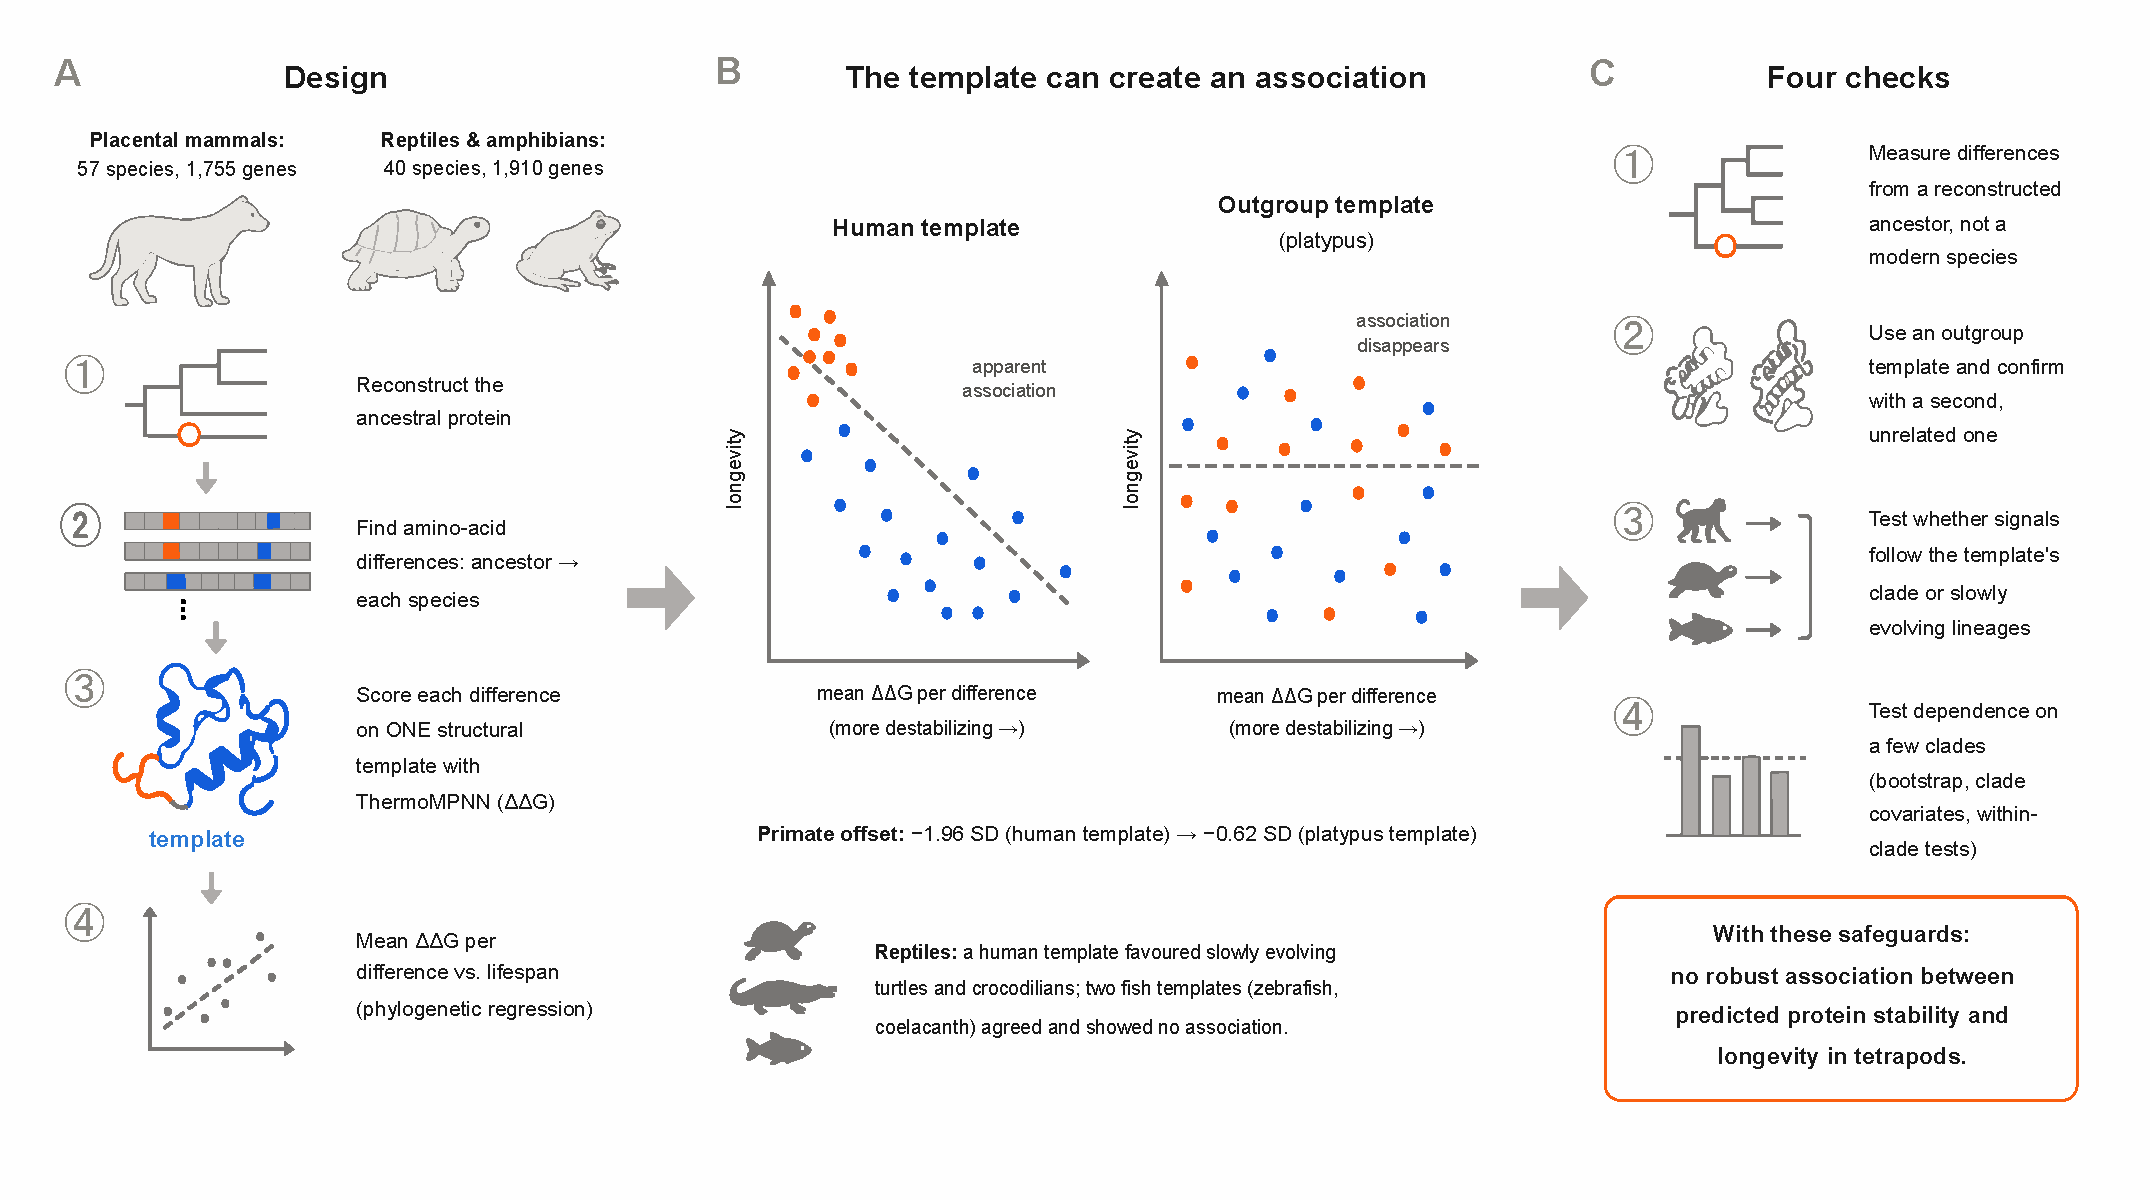
\includegraphics[width=\textwidth]{figures/fig_overview.pdf}
\caption{Overview of the study. (A) Design of the two comparative studies. (B) How the structural template can create an apparent association with longevity; the scatter plots are schematic and do not show data, whereas the primate offsets are those of the confirmatory test (Section~\ref{sec:mammaltemplates}). (C) The four checks proposed to detect this bias.}
\label{fig:overview}
\end{figure}

\section{Methods}

\subsection{Design and pre-specified plans}
Both studies followed the same logic (Table~\ref{tab:design}). For each species and gene, we identified the amino-acid differences between a reconstructed ancestor and the extant protein and predicted their effect on folding stability on a single structural backbone; species-level summaries were then related to lifespan. Each study had an internal analysis plan written before protein, ortholog or structure data were retrieved, and dated amendments were recorded. Plans were hashed with SHA256 at each stage; the hashes show that their contents were not altered afterwards but do not independently certify when they were written, and neither plan was deposited in a public registry. In the mammal study, three operational amendments preceded all association tests, one analysis (an opossum template) was added after the primary results were known and is labelled post hoc, and one confirmatory amendment (E5, a platypus template) was specified before any of its data were retrieved. In the reptile and amphibian study, a single operational amendment preceded all tests; its design incorporated the lessons of the mammal study. Software versions, data releases with retrieval dates, genome assemblies and all fixed parameters are given in the Supplementary Methods (Tables~\ref{tab:software}--\ref{tab:assembliesR}).

\begin{table}[tbp]
\centering
\caption{Design of the two studies.}
\label{tab:design}
\small
\begin{tabularx}{\textwidth}{p{3.3cm}YY}
\toprule
 & Study 1: placental mammals & Study 2: reptiles and amphibians \\
\midrule
Species analysed & \MNSpecies{} placentals (10 orders) & \RNSpecies{} (\RNTurtles{} turtles, \RNCrocs{} crocodilians, \RNSquamates{} squamates, \RNAmphibians{} amphibians) \\
Genomes and orthologs & Ensembl 116, Compara one-to-one & NCBI RefSeq, NCBI one-to-one orthologs \\
Genes & \MNGenes{} (\MNGenAge{} GenAge) & \RNGenes{} (\RNGenAge{} GenAge) \\
Alignment & Pairwise to human, anchored on human positions & MAFFT multiple alignment, anchored on the template \\
Reference ancestor & Placental ancestor & Tetrapod ancestor (amphibians + amniotes) \\
Phylogeny & Upham et al.\ MCC tree; 20 posterior trees & TimeTree 5 pairwise ages \\
Primary template & Human AlphaFold model & Zebrafish AlphaFold model (equidistant from all tetrapods) \\
Template checks & Mouse (pre-specified); opossum (post hoc); platypus (confirmatory); platypus without human anchoring (post hoc) & Coelacanth (all species); human (reptiles only) \\
Body mass & AnAge & AnAge; AmphiBIO or ReptTraits if missing \\
\bottomrule
\end{tabularx}
\end{table}

\subsection{Species and phenotypes}
Maximum recorded lifespan and adult mass came from AnAge \citep{deMagalhaes2024} (quality ``acceptable'' or ``high'', sample size other than ``tiny''), matched by binomial or by exact-binomial NCBI Taxonomy synonyms of the same taxon. Relative longevity (LQ) in mammals was lifespan divided by $4.88\,M^{0.153}$ \citep{deMagalhaes2007}. In Study~1, genomes were the Ensembl 116 mammal assemblies \citep{Dyer2025} matching AnAge and the dated tree of \citet{Upham2019}; eight placentals with early low-coverage assemblies failed the ortholog-coverage filters, leaving \MNSpecies{} species, with six marsupials and monotremes as outgroups. In Study~2, genomes were NCBI-annotated reference assemblies \citep{OLeary2024} of turtles, crocodilians, lepidosaurs and amphibians; missing masses were taken from AmphiBIO \citep{Oliveira2017} or ReptTraits \citep{Oskyrko2024}. Of \RNCandidates{} species with lifespan and mass, \RNSpecies{} passed the coverage filters; the others lacked a RefSeq annotation usable for orthology or, for the allotetraploid \emph{Xenopus laevis}, one-to-one orthologs. Divergence times among these species, zebrafish, spotted gar, coelacanth and human came from the TimeTree 5 API \citep{Kumar2022}; an average-linkage tree reproduced them exactly (root \RRootAge{} Ma). Lifespan and body mass of all species analysed are shown in Figure~\ref{fig:species} and listed, with their species-level metrics, in Tables~\ref{tab:speciesM} and \ref{tab:speciesR}.

\subsection{Genes, alignments and ancestral reconstruction}
Each study analysed human genes from GenAge \citep{deMagalhaes2024} and a background of 2,000 other genes taken in a fixed random order, with proteins of 50--1,000 residues and a full-length AlphaFold DB model \citep{Jumper2021,Varadi2024} identical to the template sequence (human in Study~1, zebrafish in Study~2). In Study~1, orthologs were aligned pairwise to the human protein (BLOSUM62, free end gaps) and anchored on human positions; in Study~2, all orthologs, three fishes and human were aligned with MAFFT \citep{Katoh2013} and columns were defined by the zebrafish residues. Eligible sites had pLDDT $\geq 70$ in the template model; species--gene pairs, genes and species were retained by coverage thresholds fixed in the plans ($\geq 80\%$ of eligible sites per pair, $\geq 60\%$ of species per gene with outgroups present, $\geq 70\%$ of genes per species). Ancestral states were inferred with IQ-TREE 2.4.0 \citep{Minh2020} under LG+G4 \citep{Le2008} on the fixed species topology, at the placental (Study~1) or tetrapod (Study~2) ancestor; mean posterior probabilities of the most probable state were 0.992 and \RAsrPost, and the ancestral node was verified independently in 60 random genes per study.

\subsection{Stability prediction and metrics}
ThermoMPNN predicts $\Delta\Delta G(a\rightarrow b)$ at site $i$ as $f_i(b)-f_i(a)$ from frozen ProteinMPNN embeddings of the backbone and full sequence. We threaded the maximum a posteriori ancestral sequence onto the template backbone and obtained $f_i$ for all sites in one pass; our vectorized implementation reproduced the original per-mutation code to within $10^{-6}$. Positive values are destabilizing. For species $s$ with residue $b$ at site $i$,
\begin{equation}
\Delta\Delta G_i(s) = f_i(b) - \sum_a P(\mathrm{anc}_i = a)\, f_i(a), \qquad K_i(s) = 1 - P(\mathrm{anc}_i = b).
\end{equation}
Positions in 10-residue windows with $\geq 5$ differences from the ancestor were masked as probable alignment or annotation errors (2.6\% of sites in Study~1; \RMaskPct\% in Study~2, where many such windows reflect true divergence). The primary metric was $M_s = \sum \Delta\Delta G/\sum K$, the mean predicted \ddG{} per amino-acid difference from the ancestor; secondary metrics were the net \ddG{} per site and the divergence per site, $R_s = \sum K/L$, the expected proportion of sites at which the species differs from the ancestor. A difference is the net outcome of all substitutions at a site along the lineage: a change followed by a reversal leaves no difference, and successive changes count once. $M_s$ and $R_s$ therefore describe net differences rather than every substitution that occurred; with at most about a tenth of the sites differing from the ancestor (mean $R_s$ \RRAmphibians{} in amphibians, the most divergent group), multiple changes at the same site should be uncommon. $M_s$ summarizes how a species' amino-acid differences from the ancestor are predicted to affect folding when each is evaluated singly, in the ancestral sequence context and on a fixed backbone. It is not a measurement of the stability of the extant proteins: effects are summed additively and epistasis is ignored. For double mutants, additive ThermoMPNN predictions perform comparably to non-additive models, but no current model captures epistasis well \citep{Dieckhaus2025}.

\subsection{Statistical analysis}
In each study, log$_{10}$ maximum lifespan was regressed on the standardized metric and log$_{10}$ adult mass by generalized least squares with Pagel's $\lambda$ estimated by maximum likelihood \citep{Pagel1999,Freckleton2002}, with likelihood-ratio tests calibrated by 999 parametric bootstrap simulations re-estimating $\lambda$. The two primary tests per study (each at $\alpha=0.025$) were P1 ($M_s$ over all genes) and P2 ($M_s$ over GenAge genes, also compared with 1,000 random background gene sets of equal size). Predictor sanity controls (C1--C3) and a positive control (divergence from the ancestor against lifespan, as a measure of the rate of protein evolution) were specified in advance. Sensitivity analyses are listed in Tables~\ref{tab:sensM} and \ref{tab:sensR}. In the mammal confirmatory amendment E5, all templates were evaluated on identical genes and sites. The primate offset $\Delta_T$ was the mean metric of primates minus that of other placentals, in SD, for template $T$. Three hypotheses were fixed with decision rules based on 1,000 bootstrap resamples of genes:
\begin{itemize}[leftmargin=*,itemsep=0pt]
\item H5a: $\Delta_\mathrm{human} - \Delta_\mathrm{platypus} < 0$;
\item H5b: the two outgroup templates agree more with each other than with the human template;
\item H5c: P1 with the platypus template gives no association (bootstrap $P \geq 0.025$ and 95\% CI including zero).
\end{itemize} Per-gene tests were exploratory, with Benjamini--Hochberg correction \citep{Benjamini1995}. After all planned results were known, three post hoc exploratory analyses were specified in dated amendments before being computed (E6 in Study~1, E2 in Study~2; Supplementary Methods). They were a reanalysis of the mammal outgroup template with alignments and sites that did not depend on the human sequence, a follow-up of a nominal human-template association in reptiles, and a calibration of the per-gene tests by simulation under the null hypothesis.

\section{Results}

\subsection{The predictor captures site-level stability signal in both radiations}
Amino-acid differences between the ancestor and extant species had lower predicted \ddG{} than the 19 possible alternatives at the same sites (mammals \MCOneObs{} vs \MCOneAlt{} kcal/mol, \MCOneFrac\% of genes; reptiles and amphibians \RCOneObs{} vs \RCOneAlt, \RCOneFrac\%), as expected under purifying selection. Alternatives were more destabilizing at buried than at exposed sites (\MCTwoBur{} vs \MCTwoExp; \RCTwoBur{} vs \RCTwoExp), and proline and glycine were the most destabilizing replacements in helices and strands (Figure~\ref{fig:controls}). These controls show that the predictor is informative at the level of sites; they do not show that differences in $M_s$ between species reflect differences in the stability of extant proteins, nor that the metric is sensitive enough to detect species-level effects of a given size. Species-level values were nevertheless highly reproducible across independent outgroup templates (Sections~\ref{sec:mammaltemplates} and \ref{sec:reptiletemplates}).

\begin{figure}[tbp]
\centering
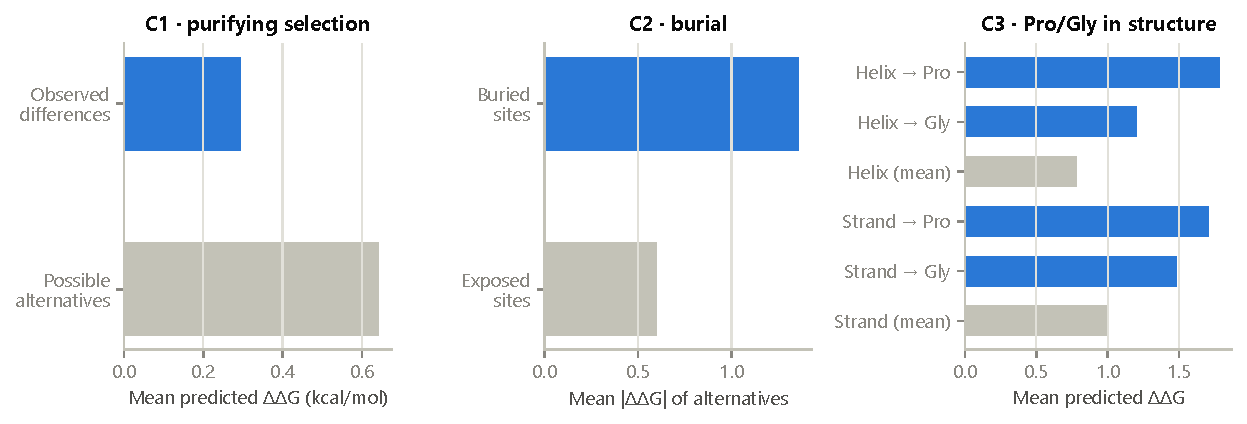
\includegraphics[width=\textwidth]{figures/mammals/fig2_controls.pdf}\\[4pt]
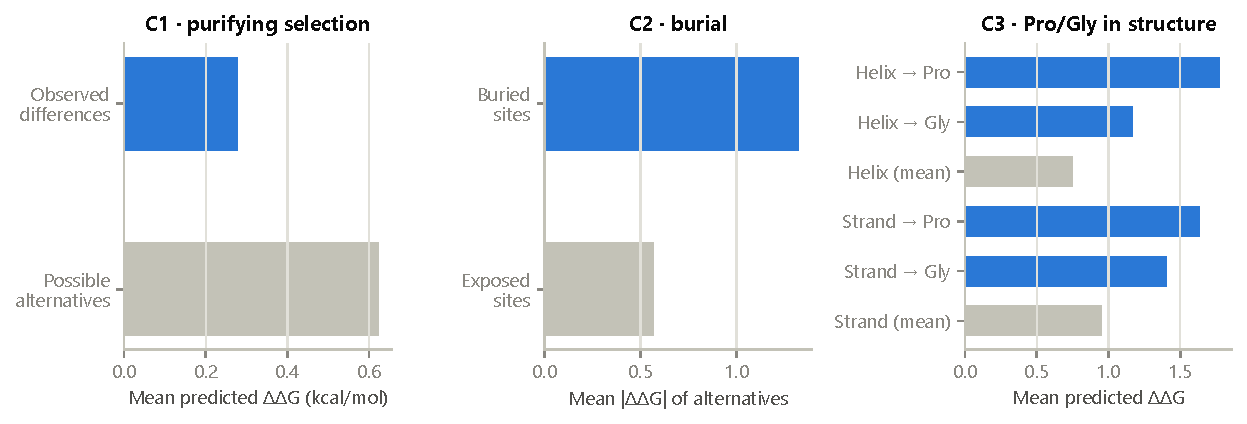
\includegraphics[width=\textwidth]{figures/ectotherms/fig2_controls.pdf}
\caption{Predictor sanity controls in placental mammals (top; human template, placental ancestor) and in reptiles and amphibians (bottom; zebrafish template, tetrapod ancestor). C1, observed differences from the ancestor vs possible alternatives at the same sites; C2, buried vs exposed sites; C3, proline and glycine replacements in helical and extended regions.}
\label{fig:controls}
\end{figure}

\subsection{No detectable association between predicted stability and lifespan}
No association between mean predicted \ddG{} per difference and lifespan was detected in mammals ($\beta$~=~\MPOneBeta{} log$_{10}$ years per SD, 95\% CI \MPOneLo{} to \MPOneHi, bootstrap $P$~=~\MPOneP) or in reptiles and amphibians ($\beta$~=~\RPOneBeta, 95\% CI \RPOneLo{} to \RPOneHi, $P$~=~\RPOneP; Table~\ref{tab:primary}, Figure~\ref{fig:primary}). Expressed as change in maximum lifespan per SD of the metric, these intervals span \MPrimaryPctLo{} to \MPrimaryPctHi{} in mammals with the human template, \MPlatypusPctLo{} to \MPlatypusPctHi{} with the platypus template on common sites (\MOpossumPctLo{} to \MOpossumPctHi{} with the opossum template), and \RPrimaryPctLo{} to \RPrimaryPctHi{} in reptiles and amphibians; they exclude large effects but remain compatible with moderate ones. Human GenAge genes and their orthologs did not differ from random background sets in either study (empirical $P$~=~\MPTwoCompP{} and \RPTwoCompP; Figure~\ref{fig:competitive}). In reptiles and amphibians, no subset showed an association: reptiles only $P$~=~\RSReptilesOnlyP, squamates only $P$~=~\RSSquamatesOnlyP, amphibians only $P$~=~\RSAmphibiansOnlyP, turtles excluded $P$~=~\RSWithoutTurtlesP. Of the remaining sensitivity analyses in both studies, only ordinary least squares without phylogeny in mammals reached $P<0.05$ ($P$~=~\MOLSP; Tables~\ref{tab:sensM} and \ref{tab:sensR}, Figure~\ref{fig:sensitivity}).

\begin{table}[tbp]
\centering
\caption{Primary and secondary tests in both studies. $\beta$ is the change in log$_{10}$ maximum lifespan per SD of the metric, adjusted for log$_{10}$ adult mass. $P$ values are parametric-bootstrap likelihood-ratio tests (999 replicates) unless marked.}
\label{tab:primary}
\small
\begin{tabularx}{\textwidth}{Yrrrr}
\toprule
Test & $\beta$ & 95\% CI & $\lambda$ & $P$ \\
\midrule
\multicolumn{5}{l}{\textit{Study 1: placental mammals ($n = \MNSpecies$)}} \\
\MPrimaryRows
\midrule
\multicolumn{5}{l}{\textit{Study 2: reptiles and amphibians ($n = \RNSpecies$)}} \\
\RPrimaryRows
\bottomrule
\end{tabularx}
\par\smallskip\raggedright\footnotesize $^{a}$Empirical two-sided $P$ against 1,000 random background gene sets of the same size. Opossum-template analyses were added after the primary results were known; platypus-template analyses follow a pre-specified confirmatory amendment and use the sites common to all three templates.
\end{table}

\begin{figure}[tbp]
\centering
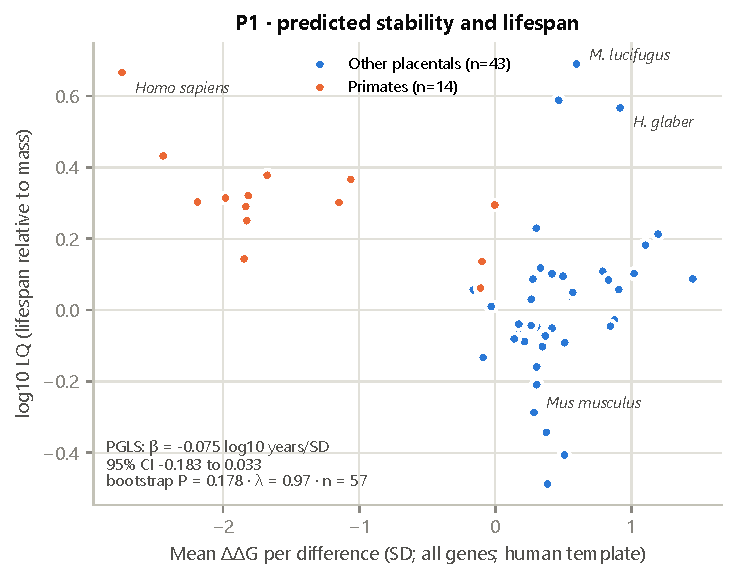
\includegraphics[width=0.7\textwidth]{figures/mammals/fig3_primary.pdf}\\[6pt]
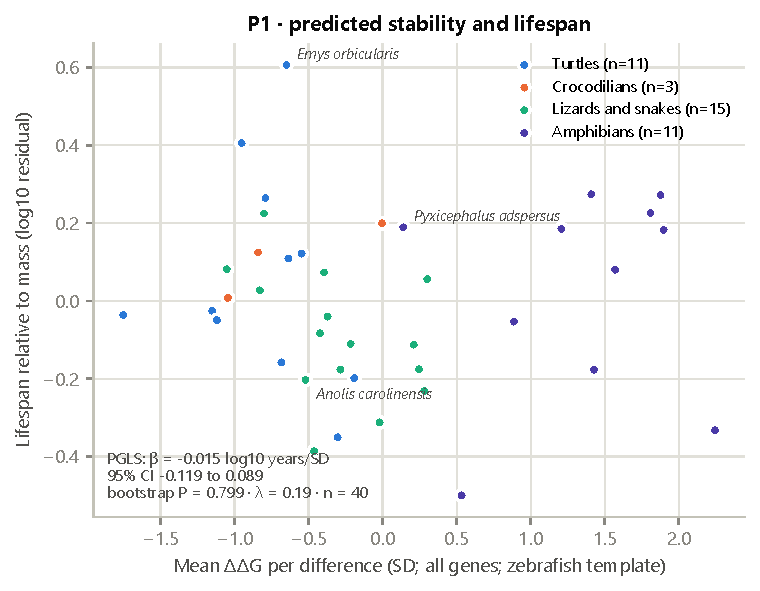
\includegraphics[width=0.7\textwidth]{figures/ectotherms/fig3_primary.pdf}
\caption{Mean predicted \ddG{} per difference from the ancestor against relative longevity. Top, placental mammals (human template; primates in orange). Bottom, reptiles and amphibians by clade (zebrafish template; lifespan residual on mass shown for display). Insets report the primary PGLS results.}
\label{fig:primary}
\end{figure}

\subsection{Template proximity drives an apparent association in mammals}
\label{sec:mammaltemplates}
With the human backbone, humans had the lowest mean \ddG{} per difference of all \MNSpecies{} mammals, followed by chimpanzee, gorilla and macaques; the primate mean lay 1.97 SD below that of other placentals (Figure~\ref{fig:primary}). Because primates are long-lived for their size, this produced a weak negative slope, which pre-specified sensitivity analyses exposed: excluding primates reversed its sign ($\beta$~=~\MExPrimBeta), excluding humans alone removed it ($\beta$~=~\MExHumBeta, $P$~=~\MExHumP), and a mouse backbone reduced it (\MMouseBetaHuman{} to \MMouseBetaMouse{} in 200 genes; Figure~\ref{fig:mouse}). After seeing these results we repeated the analysis with an opossum backbone, which is equidistant from all placentals: the slope became $\beta$~=~\MOpBeta{} (95\% CI \MOpLo{} to \MOpHi, $P$~=~\MOpP).

We then specified, before retrieving any of its data, the confirmatory amendment E5 with a platypus backbone (Figure~\ref{fig:confirm}). On \MEGenes{} genes and identical sites, the primate offset was \MEOffHum{} SD with the human template, \MEOffOpo{} with the opossum and \MEOffPla{} with the platypus. The difference $\Delta_\mathrm{human} - \Delta_\mathrm{platypus}$ was \MEaEst{} SD (95\% CI \MEaLo{} to \MEaHi), that is, the primate offset was about two-thirds smaller with the platypus template (H5a confirmed). The two outgroup templates gave almost identical species values ($r$~=~\MErOpPl), whereas each agreed only moderately with the human template ($r$~=~\MErHuPl{} and \MErHuOp; H5b confirmed), and no association with lifespan was detected ($\beta$~=~\MEcBeta, 95\% CI \MEcLo{} to \MEcHi, $P$~=~\MEcP; H5c met).

A smaller primate offset and the lowest value for humans persisted with both outgroup templates. Both outgroup analyses shared features that could favour humans: eligible sites were defined on the human model and alignments were anchored on human positions. In a post hoc analysis (amendment E6) we removed both. We realigned the orthologs of \MSixGenes{} of the \MSixGenesIn{} E5 genes with MAFFT, kept the columns of the platypus protein, defined eligible sites on the platypus model alone and reconstructed the placental ancestor again, so that no step used the human sequence or model as a reference. The primate offset was essentially unchanged: \MSixOffMsa{} SD (95\% CI \MSixOffMsaLo{} to \MSixOffMsaHi), against \MSixOffPla{} SD for the human-anchored platypus analysis on the same genes (difference \MSixDiffMsaPla, 95\% CI \MSixDiffMsaPlaLo{} to \MSixDiffMsaPlaHi). Species values were nearly identical ($r$~=~\MSixRPla). Humans were no longer the lowest: counting from the lowest value they ranked \MSixRankMsa{} of \MNSpecies{} (\MSixRankPla{} with the human-anchored analysis on these genes), and no association with lifespan was detected ($\beta$~=~\MSixBeta, 95\% CI \MSixLo{} to \MSixHi, $P$~=~\MSixP). Restricting the new analysis to sites that were also eligible in the human model changed the offset by only \MSixDiffHsMsa{} SD. Human anchoring therefore does not explain the residual primate offset. Whether it reflects a genuine property of primate proteins or another bias remains open.

\begin{figure}[p]
\centering
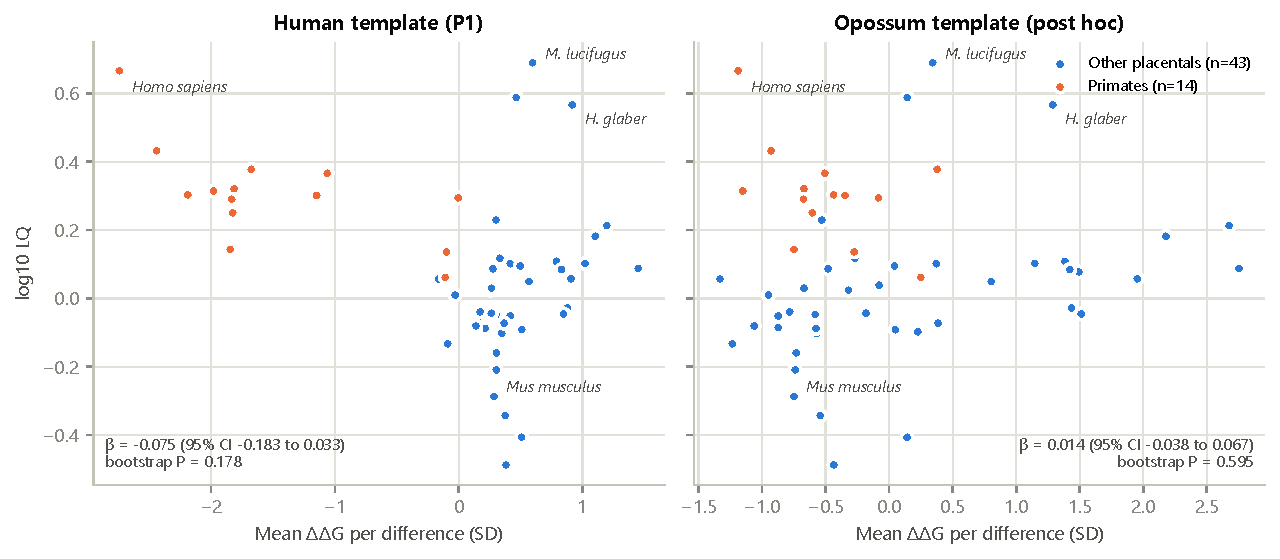
\includegraphics[width=\textwidth]{figures/mammals/fig7_template_bias.pdf}\\[14pt]
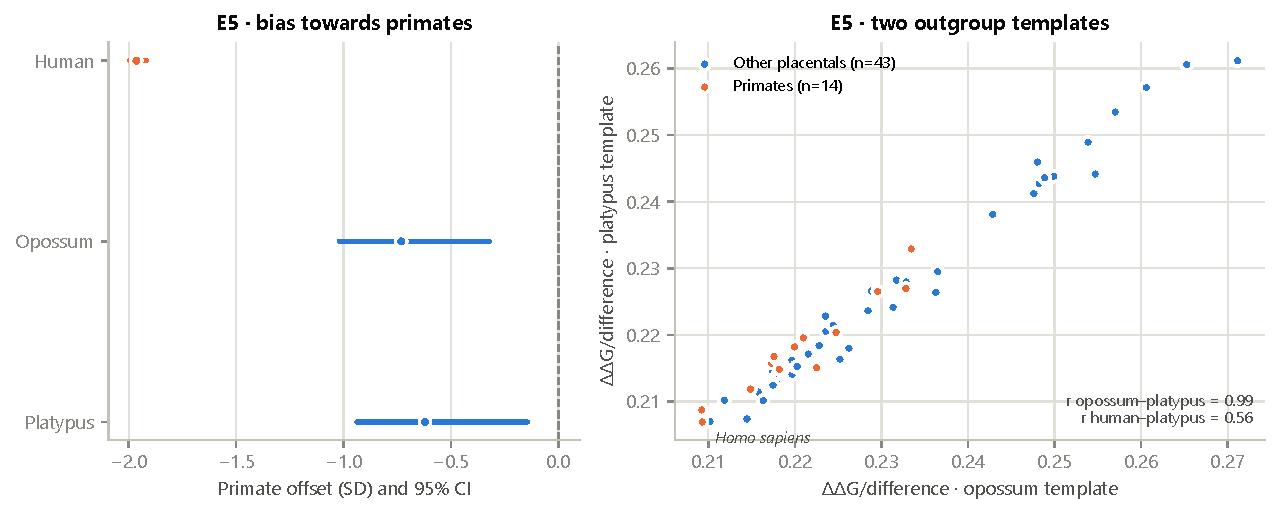
\includegraphics[width=\textwidth]{figures/mammals/fig8_confirmatory_E5.pdf}
\caption{Template bias in mammals. Top, the same species and metric with the human backbone (pre-specified primary analysis) and with the opossum backbone (post hoc). Bottom, confirmatory amendment E5 on identical genes and sites: primate offset $\Delta_T$ with each template (95\% gene-bootstrap intervals; H5a) and agreement between the opossum and platypus templates (H5b).}
\label{fig:confirm}
\end{figure}

\subsection{Equidistant in time may not be equidistant in sequence: templates in reptiles}
\label{sec:reptiletemplates}
In Study~2 the zebrafish template was chosen to be equidistant from all species. A second fish, the coelacanth, gave almost identical species values in \RTplGenes{} random genes ($r$~=~\RTplRCoel) and the same null result ($\beta$~=~\RTplBetaZf{} and \RTplBetaCoel). A human backbone is also equidistant in time from all reptiles, but within reptiles it separated slowly evolving turtles and crocodilians from faster-evolving squamates more sharply than the zebrafish backbone (Figure~\ref{fig:reptemplates}) and gave a nominal negative slope ($\beta$~=~\RTplRepHuBeta, analytic Wald $P$~=~\RTplRepHuP, with $\lambda$ estimated at \RTplRepHuLambda), against \RTplRepZfBeta{} ($P$~=~\RTplRepZfP) with zebrafish on the same genes. A $\lambda$ near zero does not by itself make an association spurious, so we examined this slope in post hoc analyses (amendment E2; Table~\ref{tab:posthocrep}). A parametric bootstrap likelihood-ratio test, which accounts for the uncertainty in $\lambda$, gave $P$~=~\RPHHuBootP. Among reptiles the human-template metric was strongly correlated with divergence from the ancestor ($r$~=~\RPHHuRRate, against \RPHZfRRate{} with zebrafish), and so was the difference between the two templates ($r$~=~\RPHDiffRRate). Adjusting for divergence halved the slope (\RPHHuRateBeta, $P$~=~\RPHHuRateP). With a clade covariate (turtles and crocodilians against squamates) the slope was similar (\RPHHuCladeBeta), but its standard error tripled (\RPHHuCladeSE; $P$~=~\RPHHuCladeP), because the metric itself largely separates the clades; these data cannot distinguish a lifespan effect from a clade effect. Within squamates the slope was \RPHHuSqBeta{} ($P$~=~\RPHHuSqP, $n$~=~\RPHHuSqN). Within turtles and crocodilians it was \RPHHuArchBeta{} ($P$~=~\RPHHuArchP, $n$~=~\RPHHuArchN; Wald test, not bootstrapped). By the criterion fixed in the amendment the result is therefore mixed: the slope lost nominal significance with the clade covariate and within squamates, but did not approach zero with the covariate and remained nominal within turtles and crocodilians. With the zebrafish template no analysis approached significance. We do not regard the human-template slope as evidence of a lifespan association. Its dependence on divergence fits a mechanism in which lineages that have changed less since the ancestor remain more compatible with a given backbone, so that a template equidistant in time can still favour slowly evolving clades.

\begin{figure}[tbp]
\centering
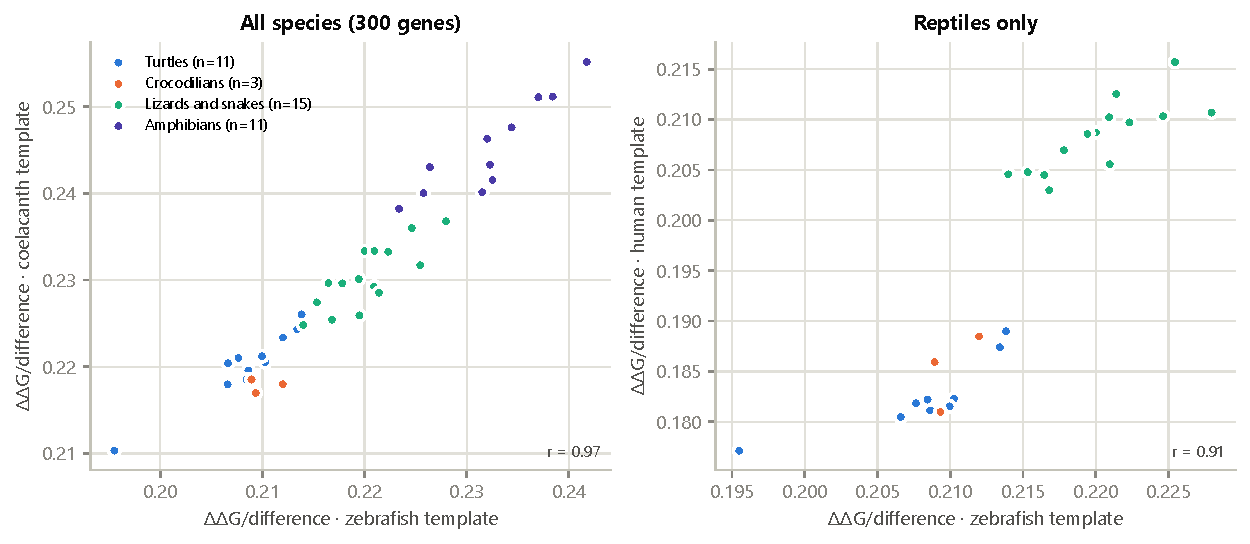
\includegraphics[width=\textwidth]{figures/ectotherms/figS1_templates.pdf}
\caption{Templates in reptiles and amphibians (\RTplGenes{} random genes). Left, coelacanth vs zebrafish backbones for all species. Right, human vs zebrafish backbones for reptiles only.}
\label{fig:reptemplates}
\end{figure}

\subsection{Clade patterns and secondary analyses}
In mammals, divergence per site from the ancestor, the positive control, was lower in longer-lived species ($\beta$~=~\MRBeta, 95\% CI \MRLo{} to \MRHi, bootstrap $P$~=~\MRP), reproducing the known association between longevity and slower molecular evolution \citep{Nabholz2008}. In reptiles and amphibians the direction was the same but not significant ($\beta$~=~\RRBeta, $P$~=~\RRP); turtles and crocodilians had the lowest divergence (\RRTurtles{} and \RRCrocodilians{} expected differences per site, vs \RRSquamates{} in squamates and \RRAmphibians{} in amphibians), consistent with their slowly evolving genomes \citep{Shaffer2013,Green2014}. The largest clade difference in the stability metric was between amphibians and reptiles (+\RAmphOffset{} SD for amphibians), which does not follow lifespan, since amphibian lifespans lie between those of squamates and turtles; turtles differed only modestly from squamates (\RTurtSqOffset{} SD). The metric was not associated with body mass in either study (mammals $P$~=~\MNNP; reptiles and amphibians $P$~=~\RNNP), so the nearly neutral prediction was not supported either.

Per-gene tests were exploratory. In mammals, one of \MGenesTested{} genes passed a false discovery rate of 5\% (NAT14, a background gene, in the direction opposite to the stability hypothesis); in reptiles and amphibians, none of \RGenesTested{} did (Figure~\ref{fig:pergene}). In Study~2, \RGenesNominal{} genes had nominal $P<0.05$ (\RGenesExpected{} expected), with \RGenesPos\% of slopes positive. A post hoc calibration (amendment E2) accounted for this excess. We simulated lifespans \RPHCalB{} times under the null model and repeated the same per-gene tests. A mean of \RPHCalMean{} genes then had $P<0.05$ (95\% interval \RPHCalLo--\RPHCalHi; false-positive rate \RPHCalFPR\%), so the observed number is compatible with no association (calibrated $P$~=~\RPHCalP; Figure~\ref{fig:calibration}). The average rate was inflated because many per-gene fits estimated $\lambda$ near zero (\RPHCalLambdaZeroPct\% below 0.05), and the interval was wide because all genes are tested against the same lifespans. With $\lambda$ fixed at the null-model value the tests were calibrated (null false-positive rate \RPHCalFixFPR\%), and \RPHCalFixObs{} genes were nominal (null mean \RPHCalFixMean, 95\% interval \RPHCalFixLo--\RPHCalFixHi). Against the simulated distributions, \RPHCalEmpGenes{} genes had empirical $P<0.05$, a number within that null range, and none passed the false discovery threshold.

\FloatBarrier
\section{Discussion}
In two independent radiations, endothermic placental mammals and ectothermic reptiles and amphibians, we did not detect an association between longevity and the mean predicted effect of the amino-acid differences that species have accumulated relative to a reconstructed ancestor, and human GenAge genes and their orthologs behaved like random background genes. In both studies the predictor distinguished observed from possible amino-acid changes and buried from exposed sites, so the predictor is not uninformative. These controls do not, however, establish that it can resolve species-level differences in the stability of extant proteins, so the null results speak to the predicted effects of these differences rather than to measured stability.

The confidence intervals limit, but do not exclude, an association. Per SD of the metric, they span \MPlatypusPctLo{} to \MPlatypusPctHi{} of maximum lifespan in mammals with an outgroup template and \RPrimaryPctLo{} to \RPrimaryPctHi{} in reptiles and amphibians, so moderate effects remain compatible with the data. For reference, the minimum effects detectable with 80\% power at the two-sided $\alpha = 0.025$ of the primary tests, computed as \PowerZ{} standard errors of $\beta$, were about \MOpDetectA\% (mammals, opossum template) and \RDetectA\% (reptiles and amphibians). Thousands of genes improve the precision of each species' estimate, but the comparative sample sizes remain \MNSpecies{} and \RNSpecies{} species. Effects confined to particular proteins or regulatory regions, and properties other than folding stability (activity, aggregation, turnover, modification), also remain open. Turtles, the clearest example of slow ageing among ectotherms \citep{daSilva2022}, did not show a distinctive folding-stability signature; their most distinctive molecular trait in our data was slow evolution.

Folding stability of isolated chains is only one layer of proteostasis. Many protein complexes are conserved across animals \citep{Wan2015}, but orthology does not guarantee that every interaction is conserved, and conservation of interactions decreases with sequence divergence \citep{Lewis2012}; subunits are also often stabilized by assembly with their partners \citep{Yeh2024}. Our metric scores each protein as a monomer, so residues at interaction interfaces, which are usually solvent-exposed in monomer models, contribute little, and compensatory substitutions between interacting partners are invisible. Longevity-related adaptation could therefore act on interfaces, complex assembly or regulation without changing the mean folding effect of amino-acid differences. A natural extension is to separate differences at known or predicted interfaces from those in the structural core, using complex structures rather than monomers and without assuming that the human interactome applies unchanged to all species.

The methodological findings may be the most broadly useful. Structure-based predictors evaluate amino-acid changes in the context of one backbone, and that backbone carries the imprint of the sequences it was predicted for. In mammals, a human backbone made primates, which are long-lived for their size, appear least destabilized, which mimicked support for the stability hypothesis. In reptiles, a human backbone, although equidistant in time, appeared to favour slowly evolving and long-lived turtles and crocodilians, and the metric it produced tracked divergence from the ancestor. \citet{Farre2021} compared FoldX energies of modelled human and rat proteins for 40 pairs and larger reference sets, with a different metric and design. Our results do not show that their conclusion is biased, but they indicate that comparisons of this kind should be checked for sensitivity to the structural template. We suggest four checks for comparative structure-based analyses:
\begin{enumerate}[leftmargin=*,itemsep=0pt]
\item measure amino-acid differences from a reconstructed ancestor, not from a modern reference species;
\item use a template outside the clade analysed and confirm results with a second, unrelated outgroup template;
\item test whether apparent associations follow the clade of the template species or slowly evolving lineages;
\item test how much an association depends on contrasts between a few clades, for example with bootstrap tests, clade covariates or within-clade analyses, particularly when $\lambda$ is estimated near zero.
\end{enumerate}

\textbf{Limitations.} ThermoMPNN predictions for single mutations are noisy and were summed additively, ignoring epistasis, protein--protein interactions, oligomers, ligands and modifications \citep{Dieckhaus2025}; the metric was not validated against measured stability differences between species. Ancestors were reconstructed, with greater uncertainty at the tetrapod node. Study~1 used human-anchored pairwise alignments and human-defined eligible sites; a post hoc reanalysis without them did not change the residual primate offset, whose origin remains unexplained. Study~2 used multiple alignments but masked more sites, partly true divergence. Species were sampled by genome availability (\MNSpecies{} and \RNSpecies), few lineages are exceptionally long-lived, AnAge records only maximum lifespans, masses in Study~2 mix typical and maximum values, and environmental temperature, which may affect both stability and ageing in ectotherms, could not be adjusted because it was available for only \RTempCov\% of reptiles, below the pre-specified threshold. The follow-up of the human template in reptiles, the calibration of the per-gene tests and the human-independent mammal reanalysis were specified after the planned results were known and are exploratory; with \RSReptilesOnlyN{} reptiles in two main clades, a clade effect and a lifespan effect cannot be separated. The opossum analysis was post hoc; its main conclusion was confirmed under a confirmatory amendment, but neither plan was deposited in a public registry, and the plan hashes document content rather than timing.

\section{Conclusion}
In two independent tetrapod radiations, the choice of structural template was enough to create an apparent association between predicted protein stability and longevity. A template from within the sample favoured the clade of the template species, and a template equidistant in time still favoured slowly evolving lineages. Ancestral references, outgroup templates and explicit checks for clade and rate effects should therefore be standard in comparative structure-based studies. We demonstrated the bias for ThermoMPNN applied to single-chain models; whether other predictors are equally sensitive remains to be tested. With these safeguards, in the proteins and \MNSpecies{} + \RNSpecies{} species analysed, we detect no robust association between longevity and the mean predicted effect on folding stability of amino-acid differences from a reconstructed ancestor; moderate effects cannot be excluded.

\section*{Declarations}
\noindent\textbf{Data and code availability.} All code, both analysis plans with their dated amendments and SHA256 hashes, the provenance log of every download (URL, retrieval date and SHA256), the result tables and the generated inputs of this manuscript are available at \url{https://github.com/Enso-bio/tetrapod-template-bias}. Downloaded inputs and large intermediate files (alignments, ancestral reconstructions and ThermoMPNN energies) are regenerated by the scripts, and TimeTree divergence times are re-queried rather than redistributed. The plan hashes verify integrity; independent evidence of when the plans were written would require a public registry.

\noindent\textbf{Funding.} This research received no specific funding.

\noindent\textbf{Competing interests.} The authors declare no competing interests.

\bibliographystyle{unsrtnat}
\bibliography{references,extra_refs}

\clearpage
\appendix
\renewcommand{\thetable}{S\arabic{table}}
\renewcommand{\thefigure}{S\arabic{figure}}
\setcounter{table}{0}
\setcounter{figure}{0}
\section*{Supplementary material}

\subsection*{Supplementary Methods}
The tables and values in this section were generated from the project files (recorded package versions, download logs and code) rather than typed by hand. Every download was logged with its URL, UTC retrieval time and the SHA256 of the stored file. Both studies ran in the same Python environment (\RunPlatform). Software and versions are listed in Table~\ref{tab:software}, and data sources with their retrieval dates in Table~\ref{tab:data}.

\begin{table}[htbp]
\centering
\caption{Software and versions.}
\label{tab:software}
\small
\begin{tabularx}{\textwidth}{p{4.2cm}p{4.4cm}Y}
\toprule
Software & Version & Use \\
\midrule
\SoftwareRows
\bottomrule
\end{tabularx}
\end{table}

\begin{table}[htbp]
\centering
\caption{Data sources. Retrieval dates are UTC ranges over both studies; the Study column gives the studies that used each source.}
\label{tab:data}
\small
\begin{tabularx}{\textwidth}{p{3.6cm}Yp{2.3cm}l}
\toprule
Source & Version or release & Retrieved & Study \\
\midrule
\DataRows
\bottomrule
\end{tabularx}
\end{table}

\paragraph{Genes and orthologs.} In both studies the gene universe was restricted to human proteins of 50--1,000 residues. GenAge human genes were always included, and background genes were taken in a fixed random order (NumPy generator, seed 20261008 in Study~1 and 20261009 in Study~2) until 2,000 passed the template criteria. Study~1 used the \texttt{ortholog\_one2one} homologies of the Ensembl 116 Compara files and the protein listed for each homology. The human template was the AlphaFold DB model whose sequence was identical to that protein. Study~2 used the \texttt{Ortholog} pairs relative to human in the NCBI \texttt{gene\_orthologs} file. For each gene it took the MANE Select or RefSeq Select protein when annotated, and the longest RefSeq protein otherwise. Genes required exactly one zebrafish ortholog; the zebrafish template was the longest isoform identical in sequence to a UniProtKB entry with a full-length AlphaFold DB model. Genome assemblies and annotations are listed in Tables~\ref{tab:assembliesM} and \ref{tab:assembliesR}.

\paragraph{Alignment and coverage.} In Study~1, each ortholog was aligned to the human protein with the Biopython \texttt{PairwiseAligner} in global mode with free end gaps. Scoring used BLOSUM62, gap opening $-10$ and extension $-0.5$, and the ortholog residue at each human position was retained. In Study~2, the orthologs, three fishes and human were aligned with MAFFT (\texttt{-{}-auto}, one thread), and the columns with a zebrafish residue were retained. The same pairwise settings were used to map residues onto the alternative templates (mouse, opossum, platypus, coelacanth and human). A species--gene pair was valid if $\geq 80\%$ of the eligible template sites (pLDDT $\geq 70$) were aligned. A gene was retained if it was valid in $\geq 60\%$ of the analysed species and also present in at least one of the six marsupial and monotreme outgroups (Study~1) or in $\geq 2$ of the 3 fishes (Study~2). Species were retained if they were valid in $\geq 70\%$ of the retained genes.

\paragraph{Trees and ancestral reconstruction.} In Study~1 the node-dated MCC tree of \citet{Upham2019} was pruned to the analysed species and outgroups, and Nexus annotations were removed. In Study~2 the tree was the average-linkage (UPGMA) tree of TimeTree pairwise ages; its maximum deviation from the queried ages was below $10^{-12}$~Ma. For each gene the tree was pruned to the species present, and IQ-TREE was run as \texttt{-te} \emph{tree} \texttt{-m LG+G4 -asr -nt 1 -seed} \emph{seed}. The topology was fixed and the branch lengths were re-estimated. The ancestral node (placental or tetrapod ancestor) was the most recent common ancestor of the ingroup in the IQ-TREE output tree rooted on the outgroups. In 60 random genes per study this node was identified independently by re-rooting with Biopython, and all agreed. The maximum a posteriori ancestral sequence was threaded onto the template, and the full posterior distribution of ancestral states entered $\Delta\Delta G_i(s)$ and $K_i(s)$.

\paragraph{Structural quantities and ThermoMPNN.} pLDDT values were read from the B-factor column of each AlphaFold model. Solvent accessibility was computed on the template model with the Biopython Shrake--Rupley algorithm \citep{Shrake1973} (100 points per atom, probe radius 1.4~\AA). It was normalised by the theoretical maximum accessibilities of \citet{Tien2013}, and sites with relative accessibility $<0.25$ were classified as buried. ThermoMPNN used the published default weights (file \texttt{thermoMPNN\_default.pt}, SHA256 \ThermoSHA) on frozen ProteinMPNN \texttt{v\_48\_020} embeddings. The model configuration was the published one: the embeddings of two ProteinMPNN layers were concatenated and passed through light attention and an output network with hidden layers of 64 and 32 units. The threaded sequence replaced the model sequence while the backbone coordinates were kept; selenocysteine was scored as cysteine. A single forward pass returned the 20-value energy vector $f_i$ for every site. On test proteins, the resulting $f_i(b)-f_i(a)$ matched the original per-mutation code to within $10^{-6}$~kcal/mol. The window mask excluded all positions of any 10-residue window containing $\geq 5$ differences between the species and the ancestor.

\paragraph{Statistics.} The phylogenetic covariance $C$ was computed from the most recent common ancestor of the analysed species and scaled to a mean root-to-tip distance of 1. Pagel's $\lambda$ transformation was $V(\lambda) = \lambda C + (1-\lambda)\,\mathrm{diag}(C)$. Generalized least squares used the eigen-decomposition of the correlation matrix, so that each value of $\lambda$ required only a weighted least-squares fit. The profile likelihood of $\lambda$ was evaluated on a 41-point grid over $[0,1]$. It was then refined by bounded Brent optimisation (tolerance $10^{-4}$) between the neighbours of the best grid point, keeping the better of the two values. Confidence intervals and Wald tests used the $t$ distribution with $n-p$ degrees of freedom. For the bootstrap likelihood-ratio tests, 999 data sets were simulated under the fitted null model (coefficients, residual variance and $\lambda$). Both models were refitted to each data set with $\lambda$ re-estimated, and $P = (1 + \#\{\mathrm{LR}^* \geq \mathrm{LR}\})/(B+1)$. The competitive test recomputed the metric for 1,000 random sets of background genes of the same size as the GenAge set and refitted the PGLS model, re-estimating $\lambda$, for each set. The two-sided empirical $P$ was $(1 + \#\{|\beta^*| \geq |\beta_\mathrm{GenAge}|\})/1001$. The predictor was standardized to unit SD before fitting. Posterior-tree sensitivity in Study~1 used 20 trees evenly spaced among the 100 downloaded posterior trees. Each analysis used a seed derived from the study seed, and rerunning the metric and statistics steps reproduced all results exactly.

\paragraph{Post hoc analyses.} These analyses were written into the analysis plans as dated amendments (E6 in Study~1, E2 in Study~2), and the plans were hashed before any of them was computed. In E6 the input genes were the \MSixGenesIn{} common genes of E5. For each gene the Compara one-to-one proteins of the \MNSpecies{} placentals and six outgroups, with human as one more species, were aligned with MAFFT (\texttt{-{}-auto}). The columns with a platypus residue were kept, and eligible sites were those with pLDDT $\geq 70$ in the platypus model. The coverage rules were those of the main analysis, with the gene filter applied to the \MNSpecies{} placentals and no refiltering of species; \MSixGenes{} genes were retained. The placental ancestor was reconstructed with the same IQ-TREE settings (mean posterior of the most probable state \MSixPost), threaded onto the platypus model and scored with ThermoMPNN and the same window mask. Primate offsets were compared with those of E5 on the same genes by 1,000 paired bootstrap resamples of genes (seed 20261070), and P1 was tested with 999 bootstrap simulations (seed 20261071). In E2(a), the species metrics of the template sensitivity analysis (\RTplGenes{} genes, \RSReptilesOnlyN{} reptiles) were used. They were analysed with bootstrap likelihood-ratio tests (999 simulations; seeds 20261080 and 20261081), with a clade covariate (turtles and crocodilians against squamates), within clades, and with adjustment for log$_{10}$ divergence from the ancestor over all genes (Table~\ref{tab:posthocrep}). In E2(b), the null model (log$_{10}$ lifespan on log$_{10}$ mass; $\lambda$~=~\RPHCalNullModelLambda) was fitted to the \RNSpecies{} species. \RPHCalB{} responses were simulated from it (seed 20261082), and every per-gene test was repeated on each with the same species, $\lambda$ estimated by maximum likelihood and the Wald test. A variant fixed $\lambda$ at the null-model value. Empirical per-gene $P$ values were $(1 + \#\{P^* \leq P\})/(B+1)$.

\begin{figure}[htbp]
\centering
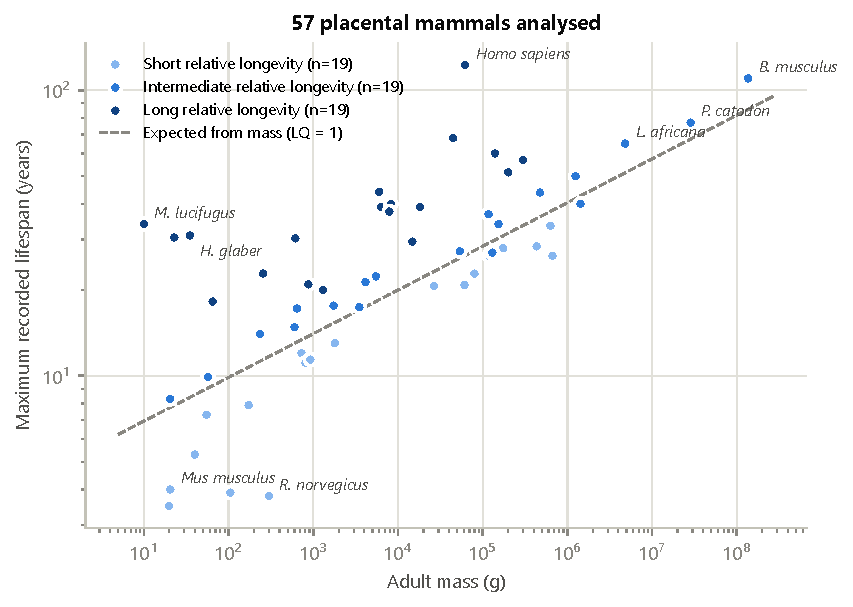
\includegraphics[width=0.49\textwidth]{figures/mammals/fig1_species.pdf}\hfill
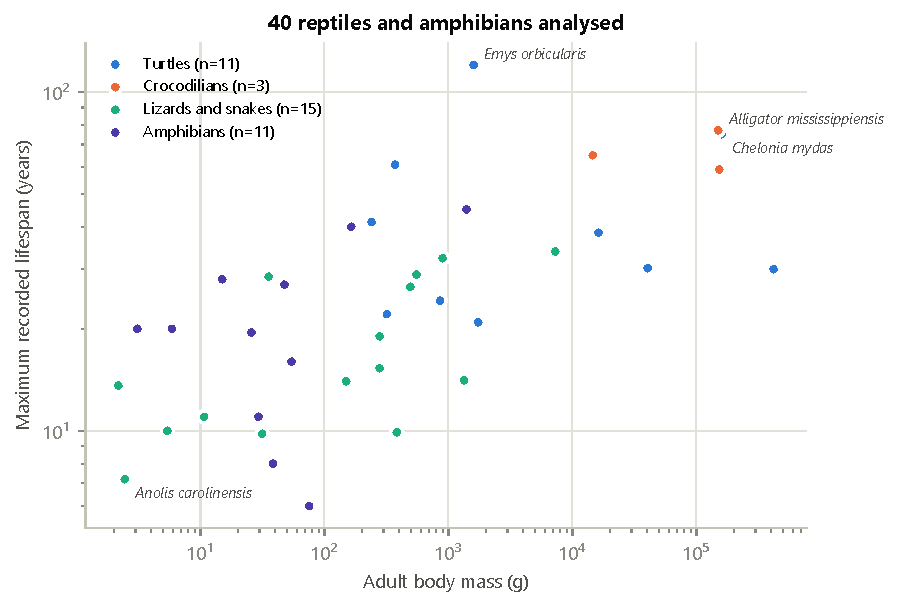
\includegraphics[width=0.49\textwidth]{figures/ectotherms/fig1_species.pdf}
\caption{Species analysed: maximum recorded lifespan against adult mass. Left, placental mammals by LQ tertile. Right, reptiles and amphibians by clade.}
\label{fig:species}
\end{figure}

\begin{figure}[htbp]
\centering
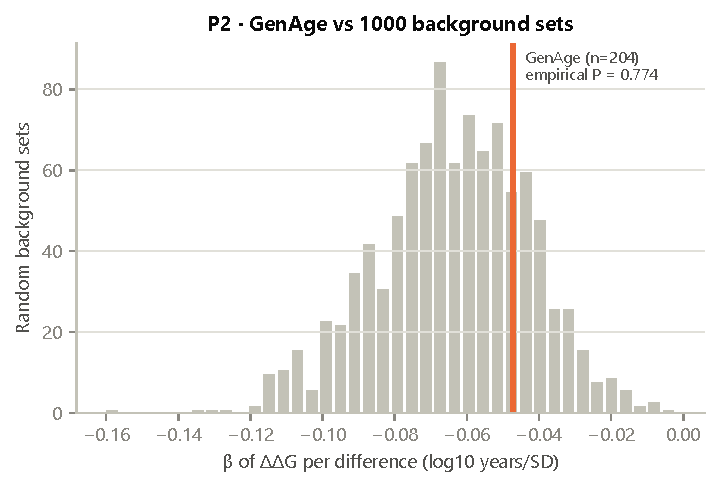
\includegraphics[width=0.49\textwidth]{figures/mammals/fig4_competitive.pdf}\hfill
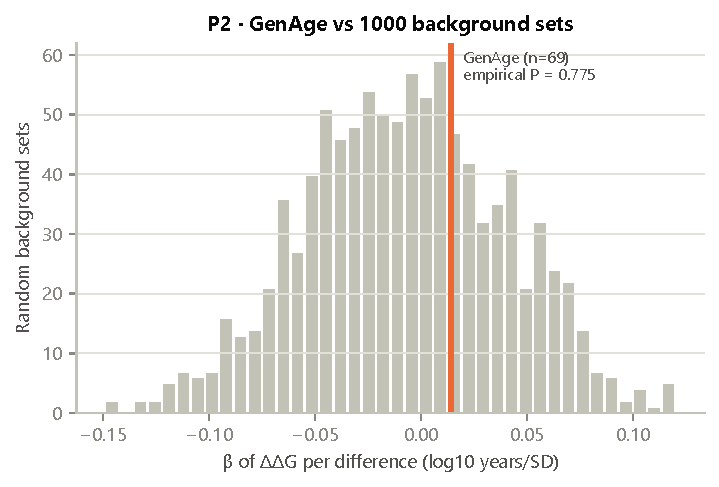
\includegraphics[width=0.49\textwidth]{figures/ectotherms/fig4_competitive.pdf}
\caption{Competitive tests of human GenAge genes and their orthologs against 1,000 random background gene sets of equal size. Left, mammals; right, reptiles and amphibians.}
\label{fig:competitive}
\end{figure}

\begin{figure}[htbp]
\centering
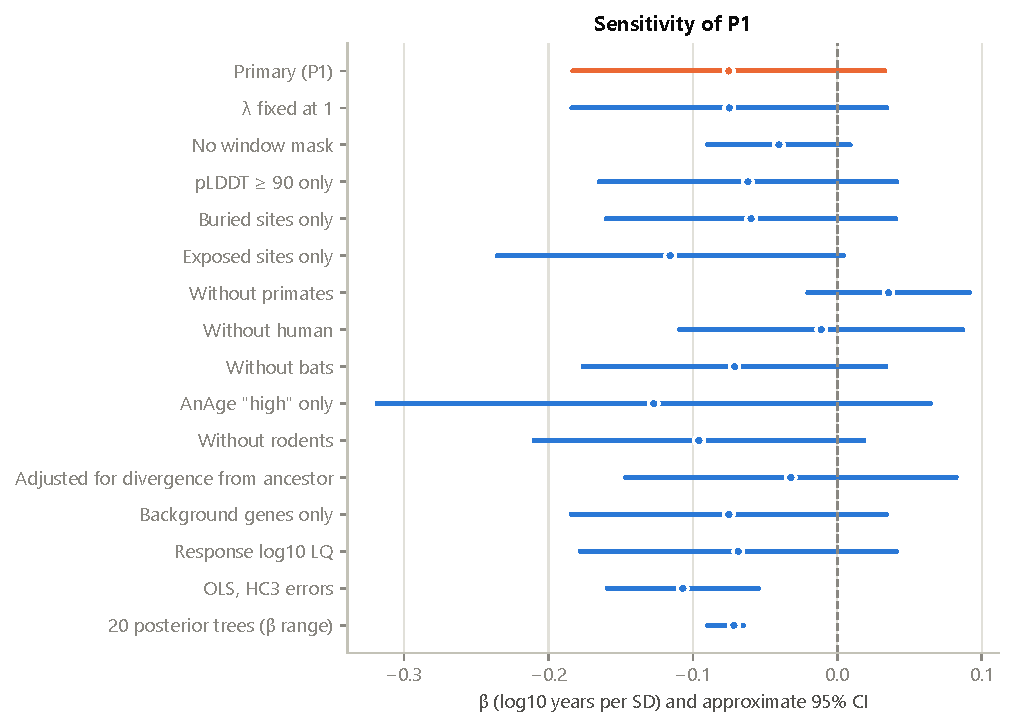
\includegraphics[width=0.66\textwidth]{figures/mammals/fig5_sensitivity.pdf}\\[6pt]
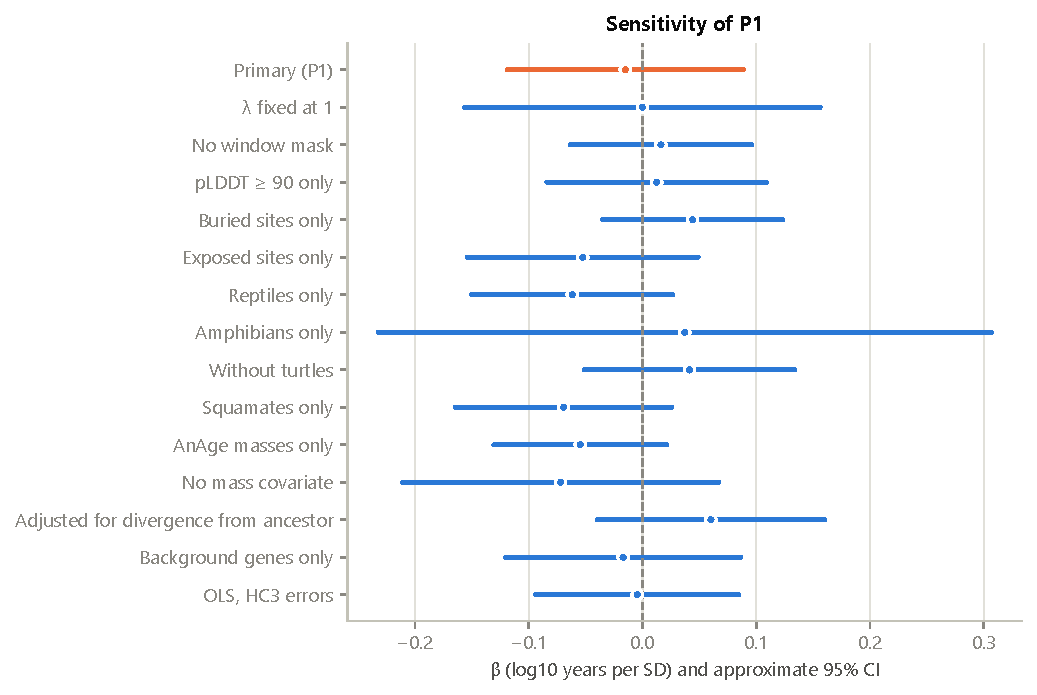
\includegraphics[width=0.66\textwidth]{figures/ectotherms/fig5_sensitivity.pdf}
\caption{Sensitivity analyses of P1. Top, mammals (last row: range over 20 posterior trees); bottom, reptiles and amphibians.}
\label{fig:sensitivity}
\end{figure}

\begin{figure}[htbp]
\centering
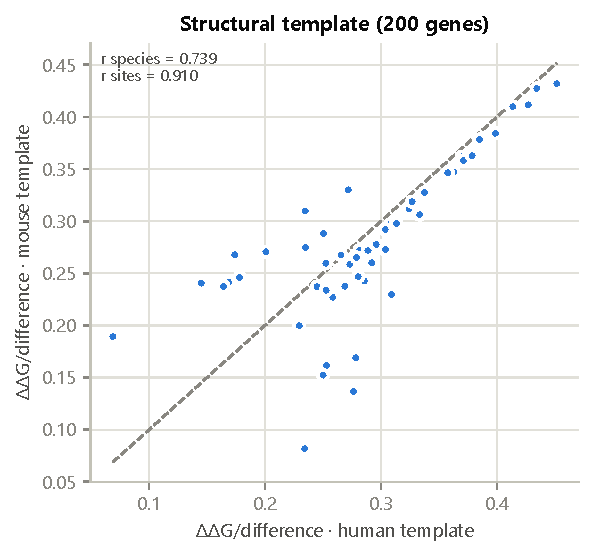
\includegraphics[width=0.5\textwidth]{figures/mammals/figS1_mouse_template.pdf}
\caption{Mammals: species-level metric with human and mouse backbones in 200 random genes (pre-specified template sensitivity).}
\label{fig:mouse}
\end{figure}

\begin{figure}[htbp]
\centering
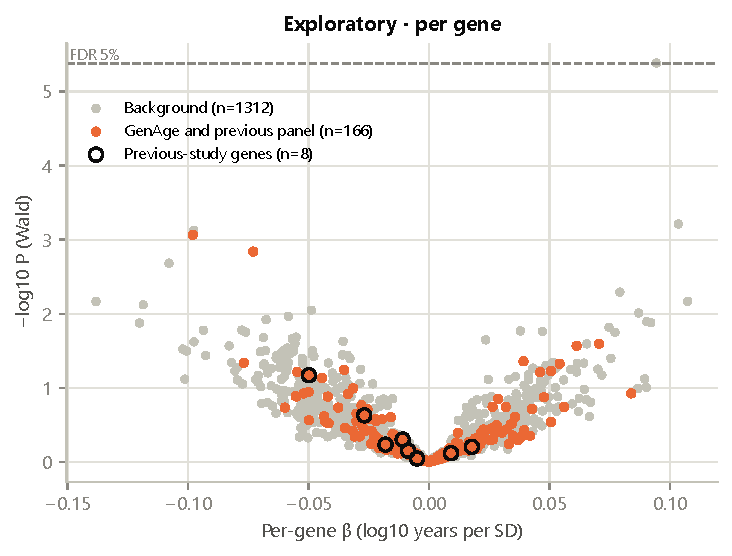
\includegraphics[width=0.49\textwidth]{figures/mammals/fig6_per_gene.pdf}\hfill
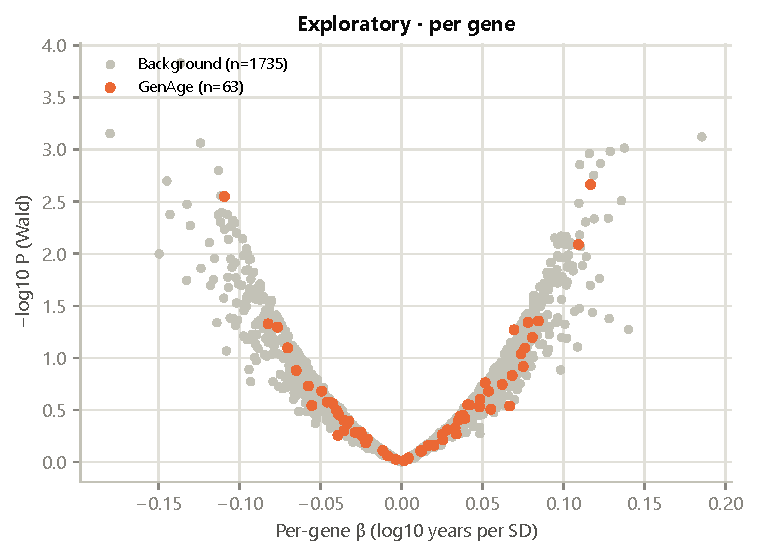
\includegraphics[width=0.49\textwidth]{figures/ectotherms/fig6_per_gene.pdf}
\caption{Exploratory per-gene tests. Left, mammals (rings: genes from a previous candidate panel); right, reptiles and amphibians.}
\label{fig:pergene}
\end{figure}

\begin{figure}[htbp]
\centering
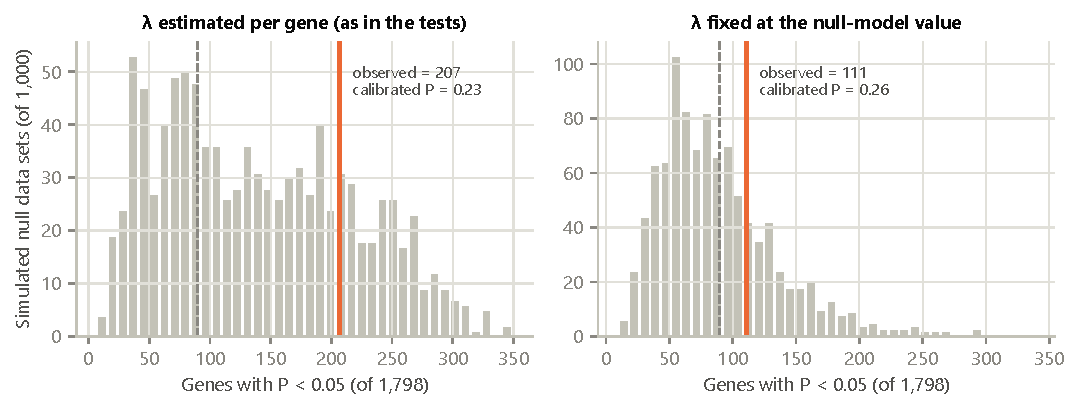
\includegraphics[width=\textwidth]{figures/ectotherms/figS3_pergene_calibration.pdf}
\caption{Post hoc calibration of the per-gene tests in reptiles and amphibians (amendment E2). Distribution of the number of genes with $P<0.05$ in \RPHCalB{} data sets simulated under the null model, with $\lambda$ estimated per gene (left) or fixed at the null-model value (right). Orange line, observed number; dashed line, 5\% of the tests.}
\label{fig:calibration}
\end{figure}

\begin{table}[htbp]
\centering
\caption{Sensitivity analyses of P1 in mammals (analytic Wald tests conditional on $\lambda$; diagnostics, not discovery tests).}
\label{tab:sensM}
\small
\begin{tabularx}{\textwidth}{Yrrrrr}
\toprule
Analysis & $n$ & $\beta$ & 95\% CI & $\lambda$ & $P$ \\
\midrule
\MSensitivityRows
\bottomrule
\end{tabularx}
\end{table}

\begin{table}[htbp]
\centering
\caption{Sensitivity analyses of P1 in reptiles and amphibians (analytic Wald tests conditional on $\lambda$).}
\label{tab:sensR}
\small
\begin{tabularx}{\textwidth}{Yrrrrr}
\toprule
Analysis & $n$ & $\beta$ & 95\% CI & $\lambda$ & $P$ \\
\midrule
\RSensitivityRows
\bottomrule
\end{tabularx}
\end{table}

\begin{table}[htbp]
\centering
\caption{Post hoc follow-up of the human-template association in reptiles (amendment E2; \RTplGenes{} genes, sites shared by the zebrafish, coelacanth and human templates). Wald tests conditional on $\lambda$ unless stated.}
\label{tab:posthocrep}
\small
\begin{tabularx}{\textwidth}{Yrrrrr}
\toprule
Analysis & $n$ & $\beta$ & 95\% CI & $\lambda$ & $P$ \\
\midrule
\RPHTemplateRows
\bottomrule
\end{tabularx}
\end{table}

\small
\setlength{\tabcolsep}{4pt}
\begin{longtable}{@{}p{4.4cm}p{2.3cm}rrrcrrr@{}}
\caption{Mammal species (names as in AnAge). Lifespan in years; mass in g; group, LQ tertile (S, I, L); $M_\mathrm{hum}$ and $M_\mathrm{opo}$, mean predicted \ddG{} per difference from the ancestor with human and opossum templates; $R$, expected proportion of sites differing from the placental ancestor.}\label{tab:speciesM}\\
\toprule
Species & Order & Lifespan & Mass & LQ & Group & $M_\mathrm{hum}$ & $M_\mathrm{opo}$ & $R$ \\
\midrule
\endfirsthead
\toprule
Species & Order & Lifespan & Mass & LQ & Group & $M_\mathrm{hum}$ & $M_\mathrm{opo}$ & $R$ \\
\midrule
\endhead
\bottomrule
\endfoot
\MSpeciesRows
\end{longtable}

\begin{longtable}{@{}p{4.6cm}p{2.4cm}rrlrr@{}}
\caption{Reptile and amphibian species (names as in AnAge). Lifespan in years; mass in g and its source; $M$, mean predicted \ddG{} per difference from the ancestor (zebrafish template); $R$, expected proportion of sites differing from the tetrapod ancestor.}\label{tab:speciesR}\\
\toprule
Species & Clade & Lifespan & Mass & Source & $M$ & $R$ \\
\midrule
\endfirsthead
\toprule
Species & Clade & Lifespan & Mass & Source & $M$ & $R$ \\
\midrule
\endhead
\bottomrule
\endfoot
\RSpeciesRows
\end{longtable}

\begin{longtable}{@{}p{4.4cm}p{5.4cm}p{5.6cm}@{}}
\caption{Study 1 genome assemblies (Ensembl 116). Species are named as in AnAge and Table~\ref{tab:speciesM}; the Ensembl genome is the one used, which for some species is a subspecies or a specific individual. Outgroups were used to root the trees and reconstruct the placental ancestor.}\label{tab:assembliesM}\\
\toprule
Species & Ensembl genome & Assembly \\
\midrule
\endfirsthead
\toprule
Species & Ensembl genome & Assembly \\
\midrule
\endhead
\bottomrule
\endfoot
\AssemblyRowsM
\end{longtable}

\begin{longtable}{@{}p{4.3cm}p{4.6cm}ll@{}}
\caption{Study 2 genome assemblies and RefSeq annotations (NCBI Datasets). Species are named as in AnAge and Table~\ref{tab:speciesR}, followed by the NCBI organism of the genome used. The reference genomes are the three fishes used as outgroups and templates and the human genome used as the orthology reference and as an alternative template.}\label{tab:assembliesR}\\
\toprule
Species & Genome (NCBI organism) & Assembly & Annotation \\
\midrule
\endfirsthead
\toprule
Species & Genome (NCBI organism) & Assembly & Annotation \\
\midrule
\endhead
\bottomrule
\endfoot
\AssemblyRowsR
\end{longtable}

\end{document}
